This section gives a background on operating system concepts such as Processes, threads, Memory protection, Virtualization and Hypervisor.

\section{Processes and threads}

\subsection{Process}

Process is a program in execution or an abstraction of a running program. Process can be called as the most central concept in an operating system. In early days, computer systems allowed only one program to be executed at a time. These programs had complete control of the system and hence could access all the resources of the system without any complications. However, modern computer systems allow multiple programs to be executed concurrently. To load and run multiple programs, operating systems require control over resource access and allocation. Isolation of the various programs is needed for resource allocation, which results in need of a process.\cite{Galvin}.
\\
A program is a passive entity, it is not a process by itself. Program is a file stored on a disk, whereas a process is an active entity, with a program counter specifying the next instruction to execute and a set of associated resources. A program becomes a process when the file is loaded into the memory\cite{Galvin}.
\\
A process is more than the program code, or the text section. It includes the current activity, with the help of the program counter and the contents of the processor's registers. A process generally also includes the process stack, which contains temporary data such as function parameters, return addresses, and local variables, and a data section, which contains global variables. A process may include a heap, which is a memory that is dynamically allocated during process run time\cite{Galvin}.
\begin{figure}[!ht]
\centering
\includegraphics[scale=.25]{Process}
\caption{Program's memory map}
\label{fig:process}
\end{figure}

\subsection{Threads}

Each process has an address space. A process has either single or multiple threads of control in that same address space. Threads run as if they were separate processes although they share the address space. \cite{Galvin}
\\
Thread is also called as a light-weight process. The implementation of threads and processes differ in each operating system, but in most cases, thread is contained inside a process. Multiple threads can exist within the same process and share resources such as code, and data segment, while different processes do not share these resources. If a process has multiple threads then it can perform more than one task at a time. 

\begin{figure}[!ht]
\centering
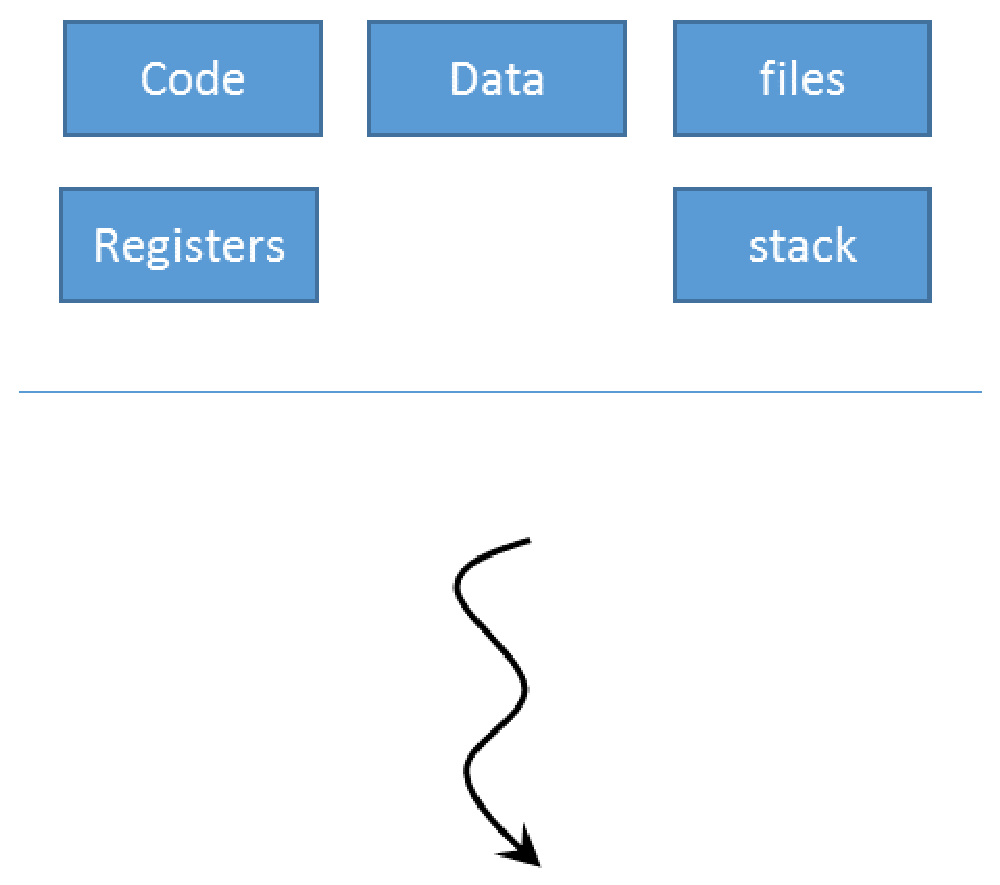
\includegraphics[scale=.25]{thread1}
\caption{Single threaded process}
\label{fig:thread1}
\end{figure}

\begin{figure}[!ht]
\centering
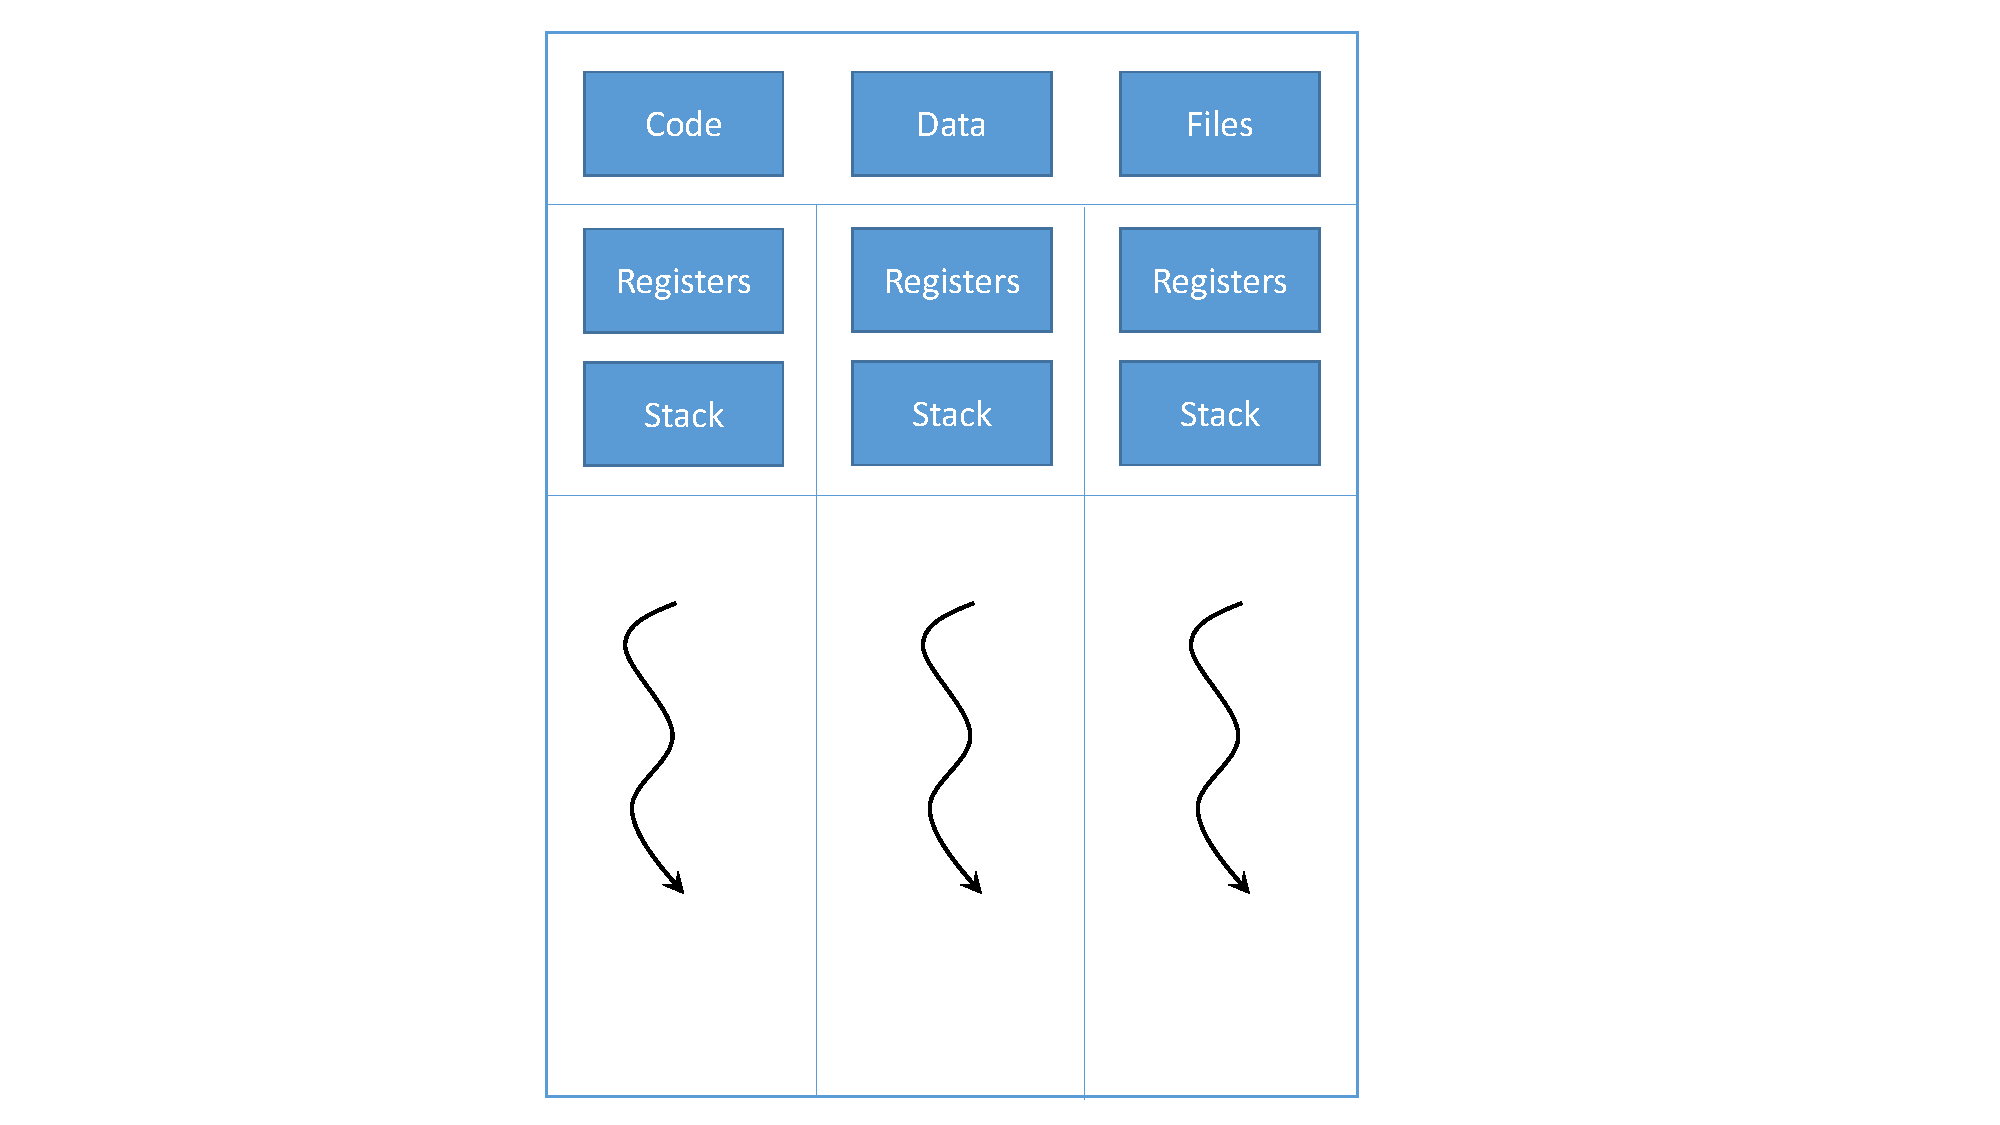
\includegraphics[scale=.25]{thread2}
\caption{Multithreaded process}
\label{fig:thread2}
\end{figure}

\subsection{Context Switch}

Multithreading is implemented by time division multiplexing on a single processor. In time division multiplexing, the processor switches between different threads. The switch between threads is called as the context switch. The context switch makes the user feel that the threads or tasks are running concurrently. However, on a multi-core system or multi-processor system, threads can run truly concurrently, with every processor or core executing a separate thread simultaneously. 
\\
In a context switch the state of a process is stored and restored, so that the execution can be resumed from the same point at a later time. The state of the process is also called as context. The context is determined by the processor and the operating system. Context switching makes it possible for multiple processes or threads to share a single processor. Usually context switches are computationally intensive. Switching between two process requires good amount of computation and time to save and load registers, memory maps, and updating various tables\cite{Galvin} .

\subsection{Spinlocks and spinning}

Spinlock is a lock which causes a thread trying to acquire it to spin continuously checking if the lock is available. Spinning is a technique in which a process repeatedly checks to see if a condition is true. Spinlock is one of the locking mechanisms designed to work in a multiprocessing environment. Spinlocks are similar to the semaphores, except that when a process finds the lock closed by another process, it spins around continuously. Spinning is implemented by executing an instruction in a loop\cite{Bovet:2005:ULK:1077084}.
\\
Whenever a lock is not available, a CPU either spins or does a context switch. In a uniprocessor environment, the waiting process keeps spinning for the lock. However, the other process holding the lock might not have a chance to release it, because of which spin lock could deteriorate the performance in a uniprocessor environment. In a multiprocessor environment, spin locks can be more efficient. Overhead for spinlocks is very small. On the other hand, a context switch takes a significant amount of time, so it is more efficient for each process to keep its own CPU and simply spin while waiting for a resource\cite{Bovet:2005:ULK:1077084}. Because spinlocks avoid overhead from operating system process re-scheduling or context switching, spinlocks are efficient if threads are only likely to be blocked for a short period. For the above reasons, spinlocks are often used inside operating system kernels.

%adaptive spinning

\pagebreak

\section{Memory protection}

The memory protection mechanism of computer systems control the access to objects. The main goal of memory protection is to prevent malicious misuse of the system by users or programs. Memory protection also ensures that each shared resource is used only in accordance with the system policies. In addition, it also helps to ensure that errant programs cause minimal damage. However, memory protection systems only provide the mechanisms for enforcing policies and ensuring reliable systems. It is up to the administrators, programmers and users to implement those mechanisms\cite{Galvin, Graham:1971:PPP:1478873.1478928}. The following subsections explain how these policies are implemented at kernel level and user level. 

\subsection{User level}

Typically in a monolithic kernel, the lowest $X$ GB of memory is reserved for user processes (In 32-bit architecture 3GB is reserved for user level). The upper $'VM - X'$ GB is reserved for kernel (In 32 bit architecture 1 GB is reserved for kernel). This upper 1 GB is restricted to $CPL 0$ $(ring 0)$ only. The kernel puts its private data structures in the upper 1GB and always accesses them at the same virtual address, irrespective of what processes are running. 
\\
\begin{figure}[!ht]
\centering
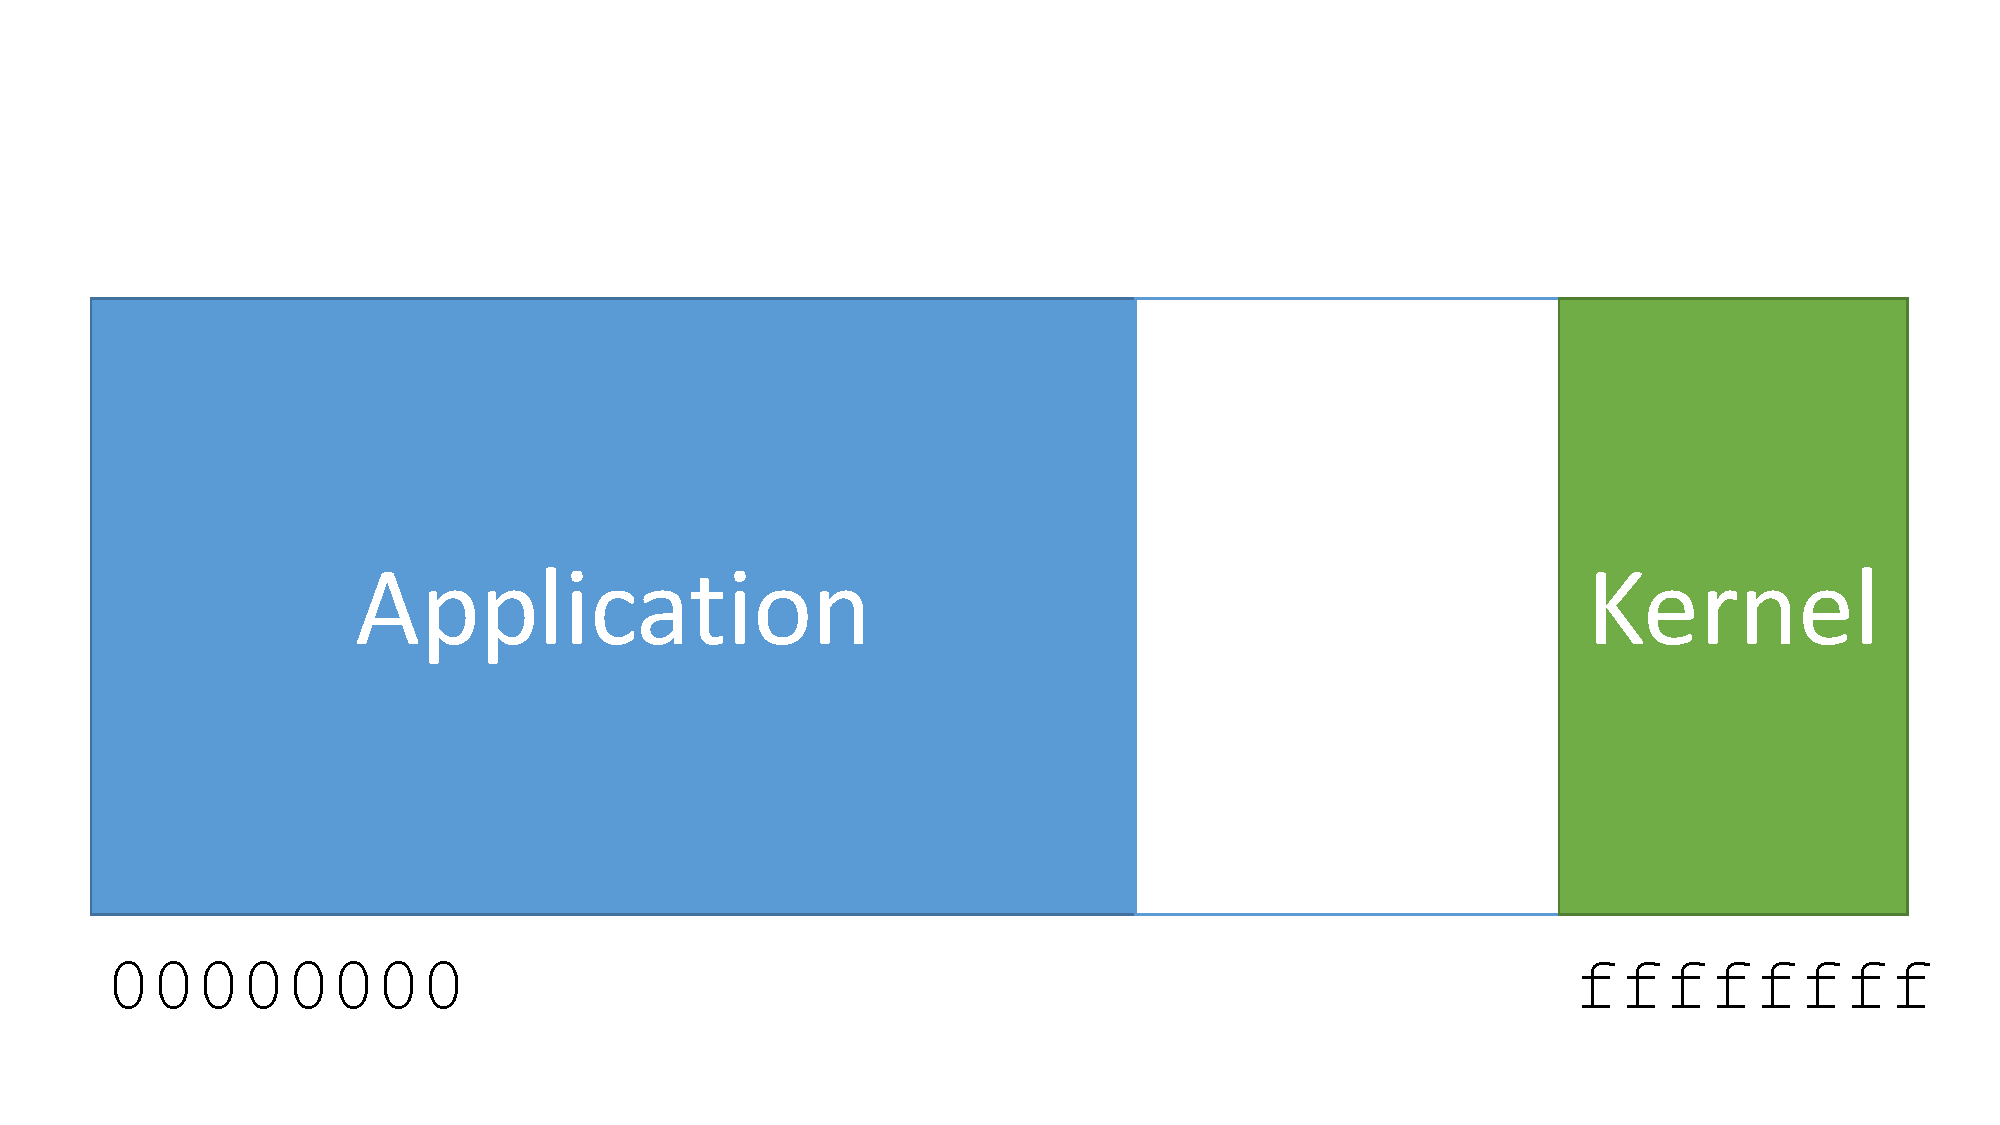
\includegraphics[scale=.25]{memory_map}
\caption{Physical memory}
\label{fig:memmap}
\end{figure}
\\
At user space, each application runs as a separate process. Each process is associated with an address space and believes that it owns the entire memory, starting with the virtual address 0.
However, a translation table translates every memory reference by these processes from virtual to physical addresses. The translation table maintains $<base, bound>$ entry. If a process tries to access virtual address which is out of $'base + bound'$ then error is reported by the OS, otherwise physical address $'base + virtual address'$ is returned. This allows multiple processes to be in memory with protection. Since address translation provides protection, a process cannot access to other processes’ addresses, nor about the OS addresses.
\\
Consider an example in below diagram.
\\*
\begin{figure}[!ht]
\centering
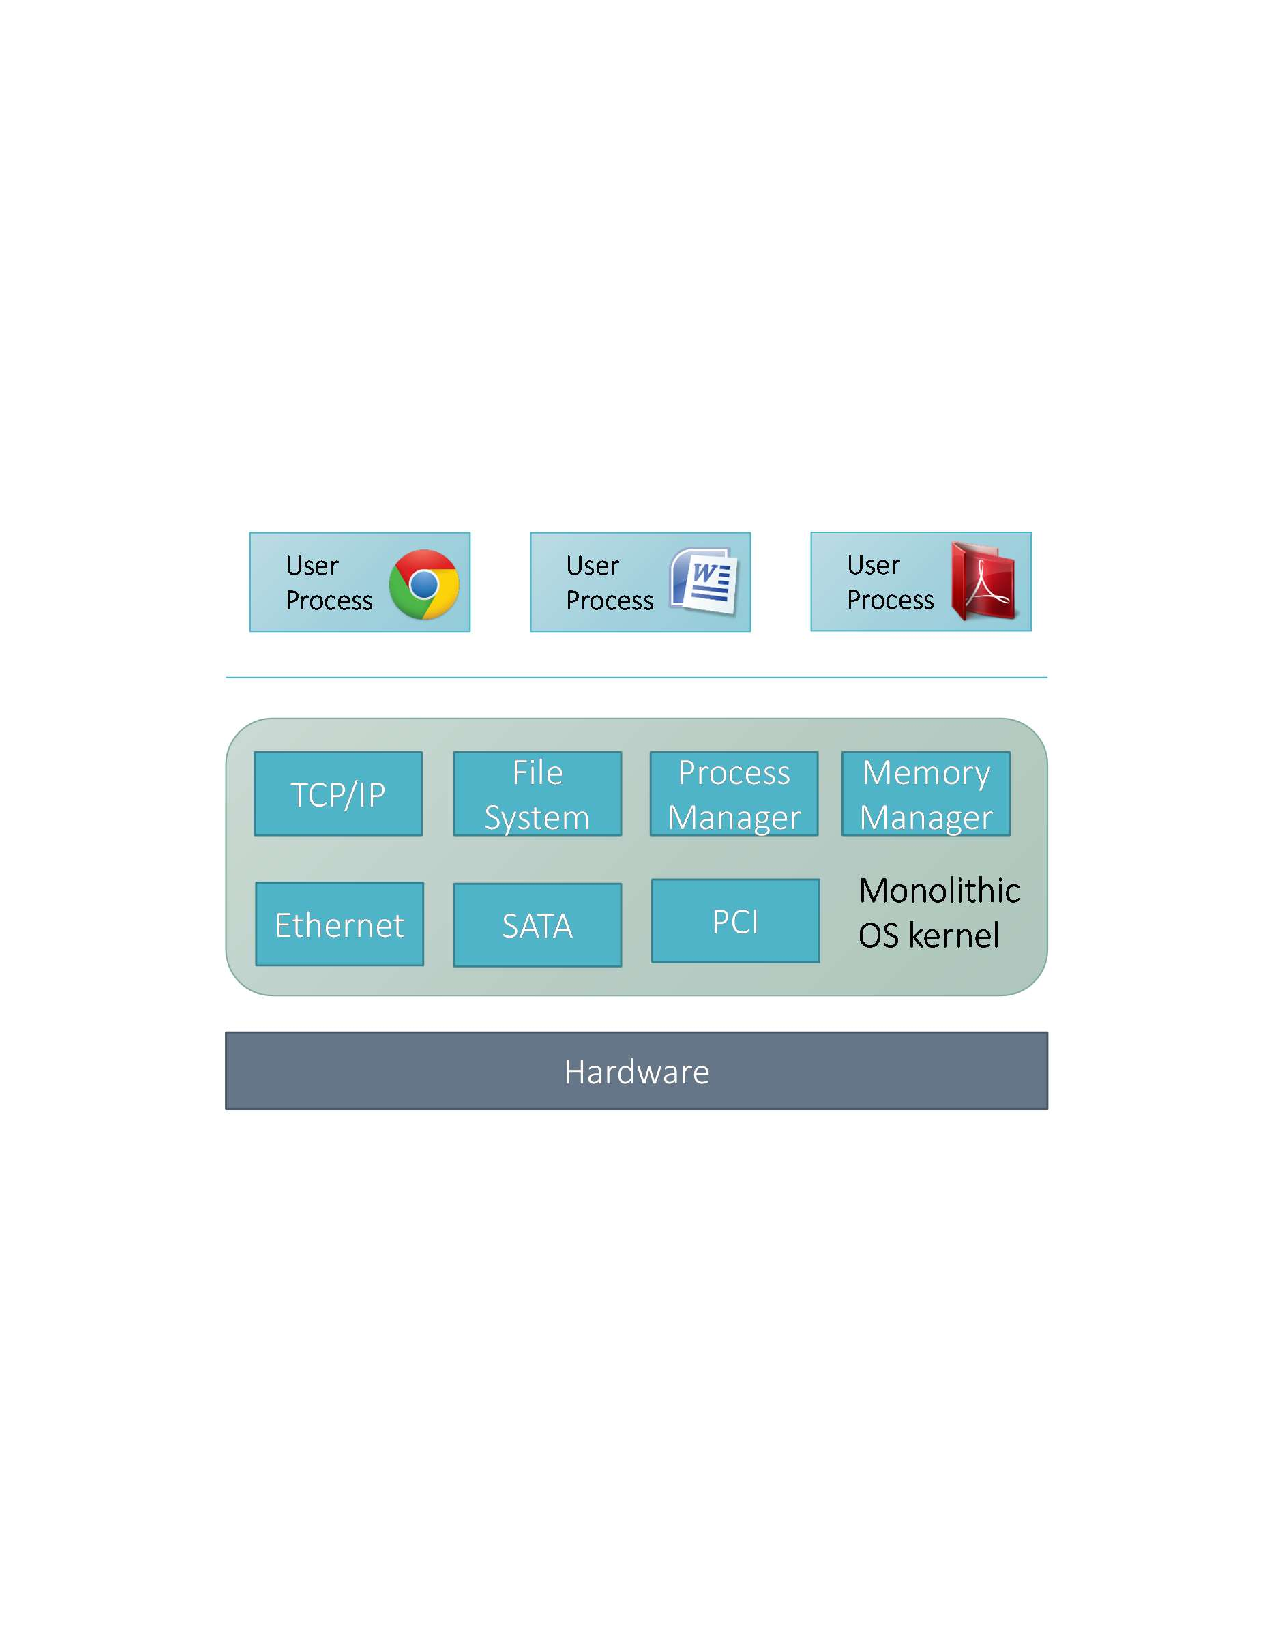
\includegraphics[scale=.5]{mem_us1}
\caption{User space}
\label{fig:User space}
\end{figure}
\begin{description}
\item In the above system Chromium browser, word processor and pdf reader are running as a 3 different processes in user space.
\item The word process hits a bug and tries to corrupt the memory out of the address space.
\item Since the access to the address is restricted because of memory protection, the word processor does not crash the other application or system.
\item The bug in the word processor might lead to crashing itself.
\end{description}
\begin{figure}[!ht]
\centering
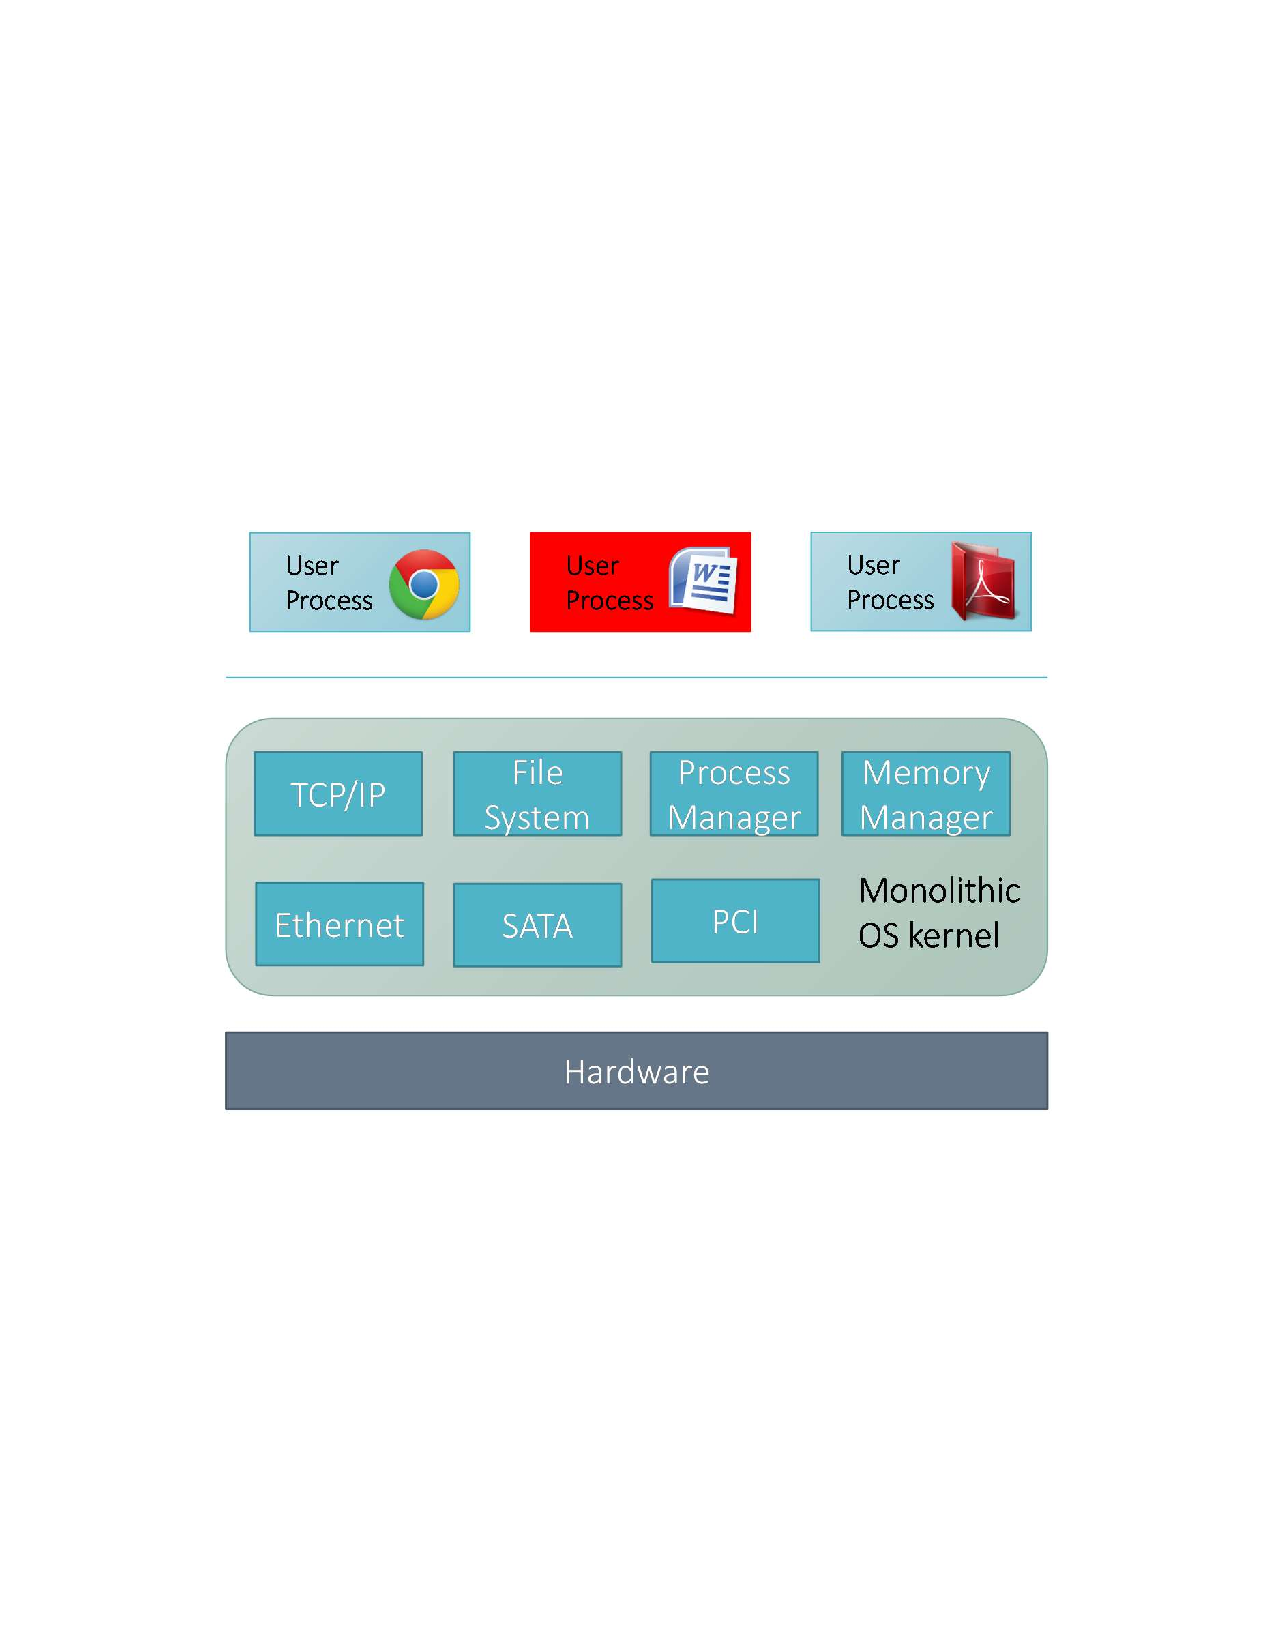
\includegraphics[scale=.5]{mem_us}
\caption{User space: Word processor hits a bug}
\label{fig:User space}
\end{figure}
\begin{figure}[!ht]
\centering
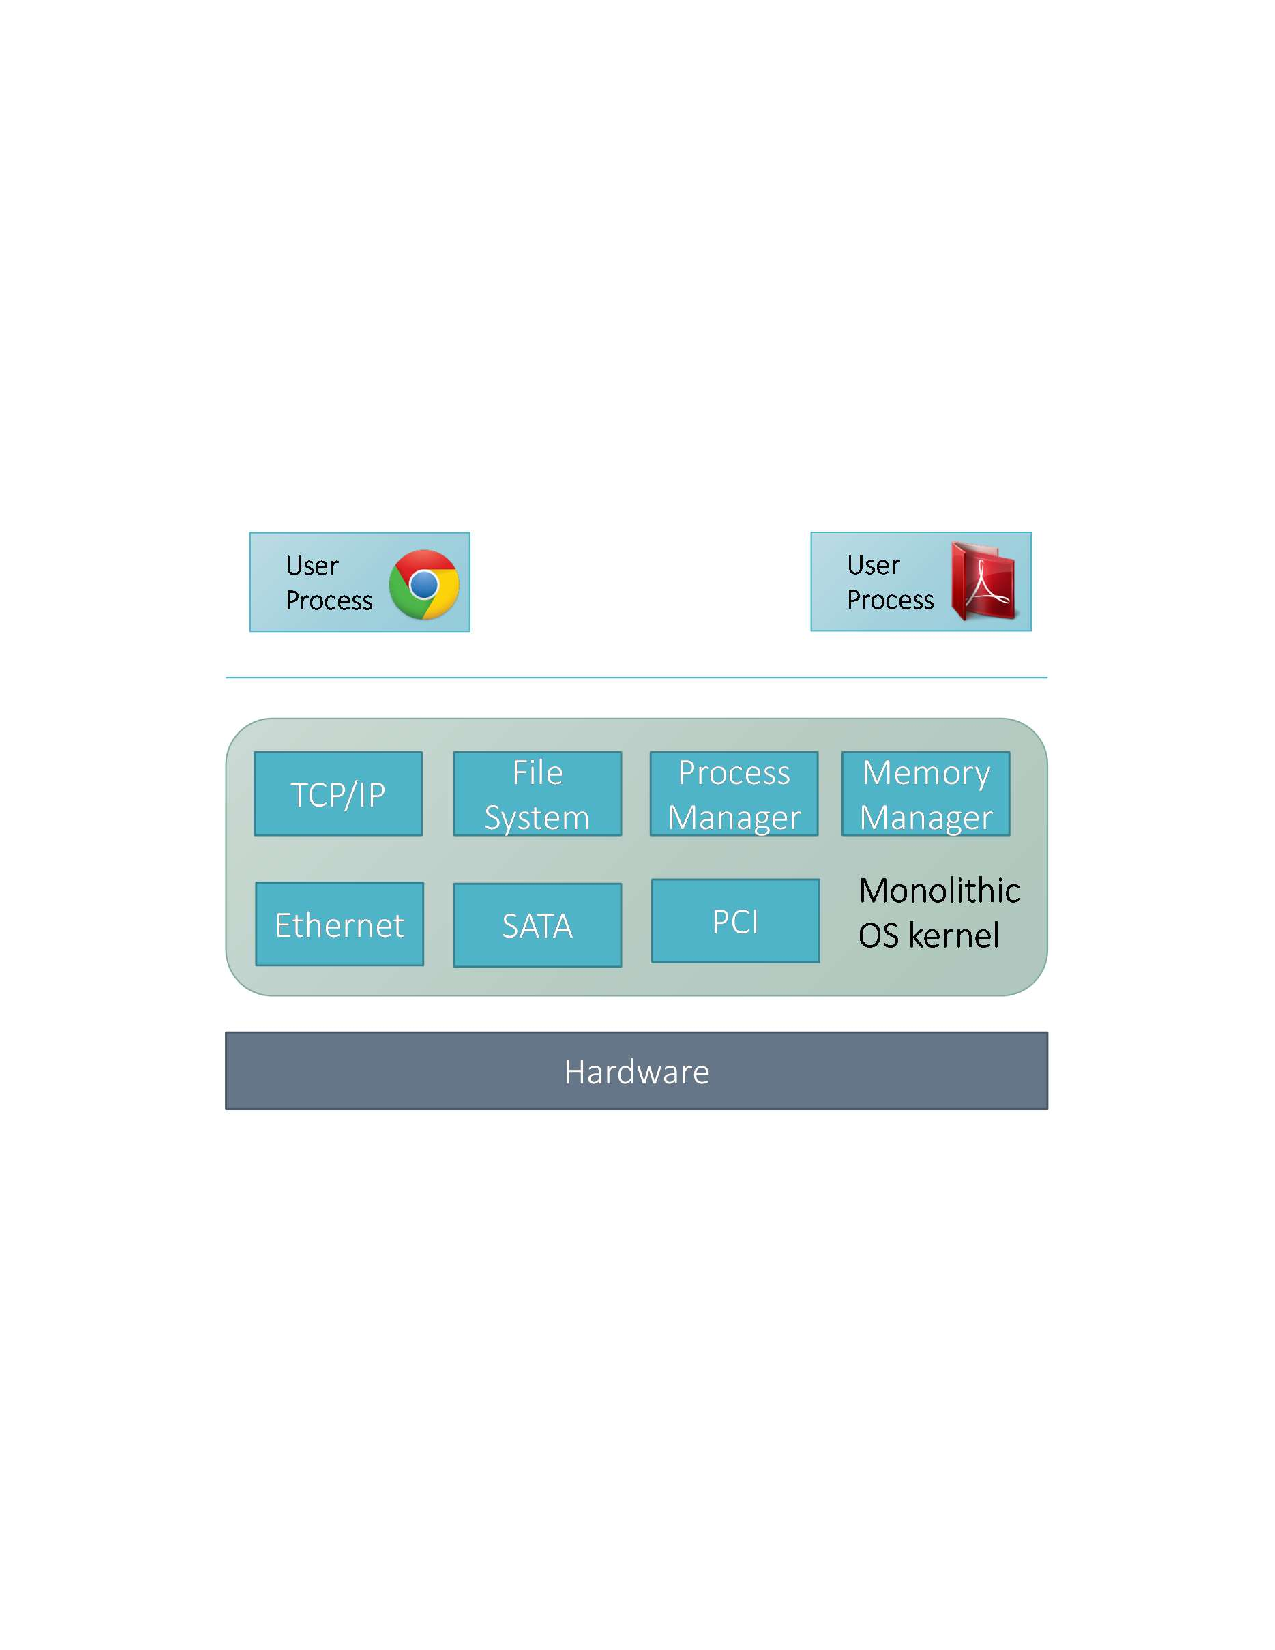
\includegraphics[scale=.5]{mem_us3}
\caption{User space : Word processor crashes and system is still intact}
\label{fig:User space}
\end{figure}

\subsection{kernel level}

Kernel reserves upper $1Gb$ of virtual memory for its internal use. The page table entries of this region are marked as protected so that pages are not visible or modifiable in the user mode. This reserved region is divided into two regions. First region contains page table references to every page in the system. It is used to do translation of address from physical to virtual when kernel code is executed. The core of the kernel and all the pages allocated by page allocator lies in this region. The other region of kernel memory is used by the memory allocator such as $vmalloc()$, the allocated memory is mapped by kernel modules using $kmap()$ or $vremap()$. Since an operating system maps physical addresses directly, kernel components do not have memory protection similar to that of the user space. At kernel level any code running at CPL 0 can access the 1 GB of kernel memory, and hence any kernel component can access and corrupt the kernel data structure. 
\\
Consider an example below.
\begin{figure}[!ht]
\centering
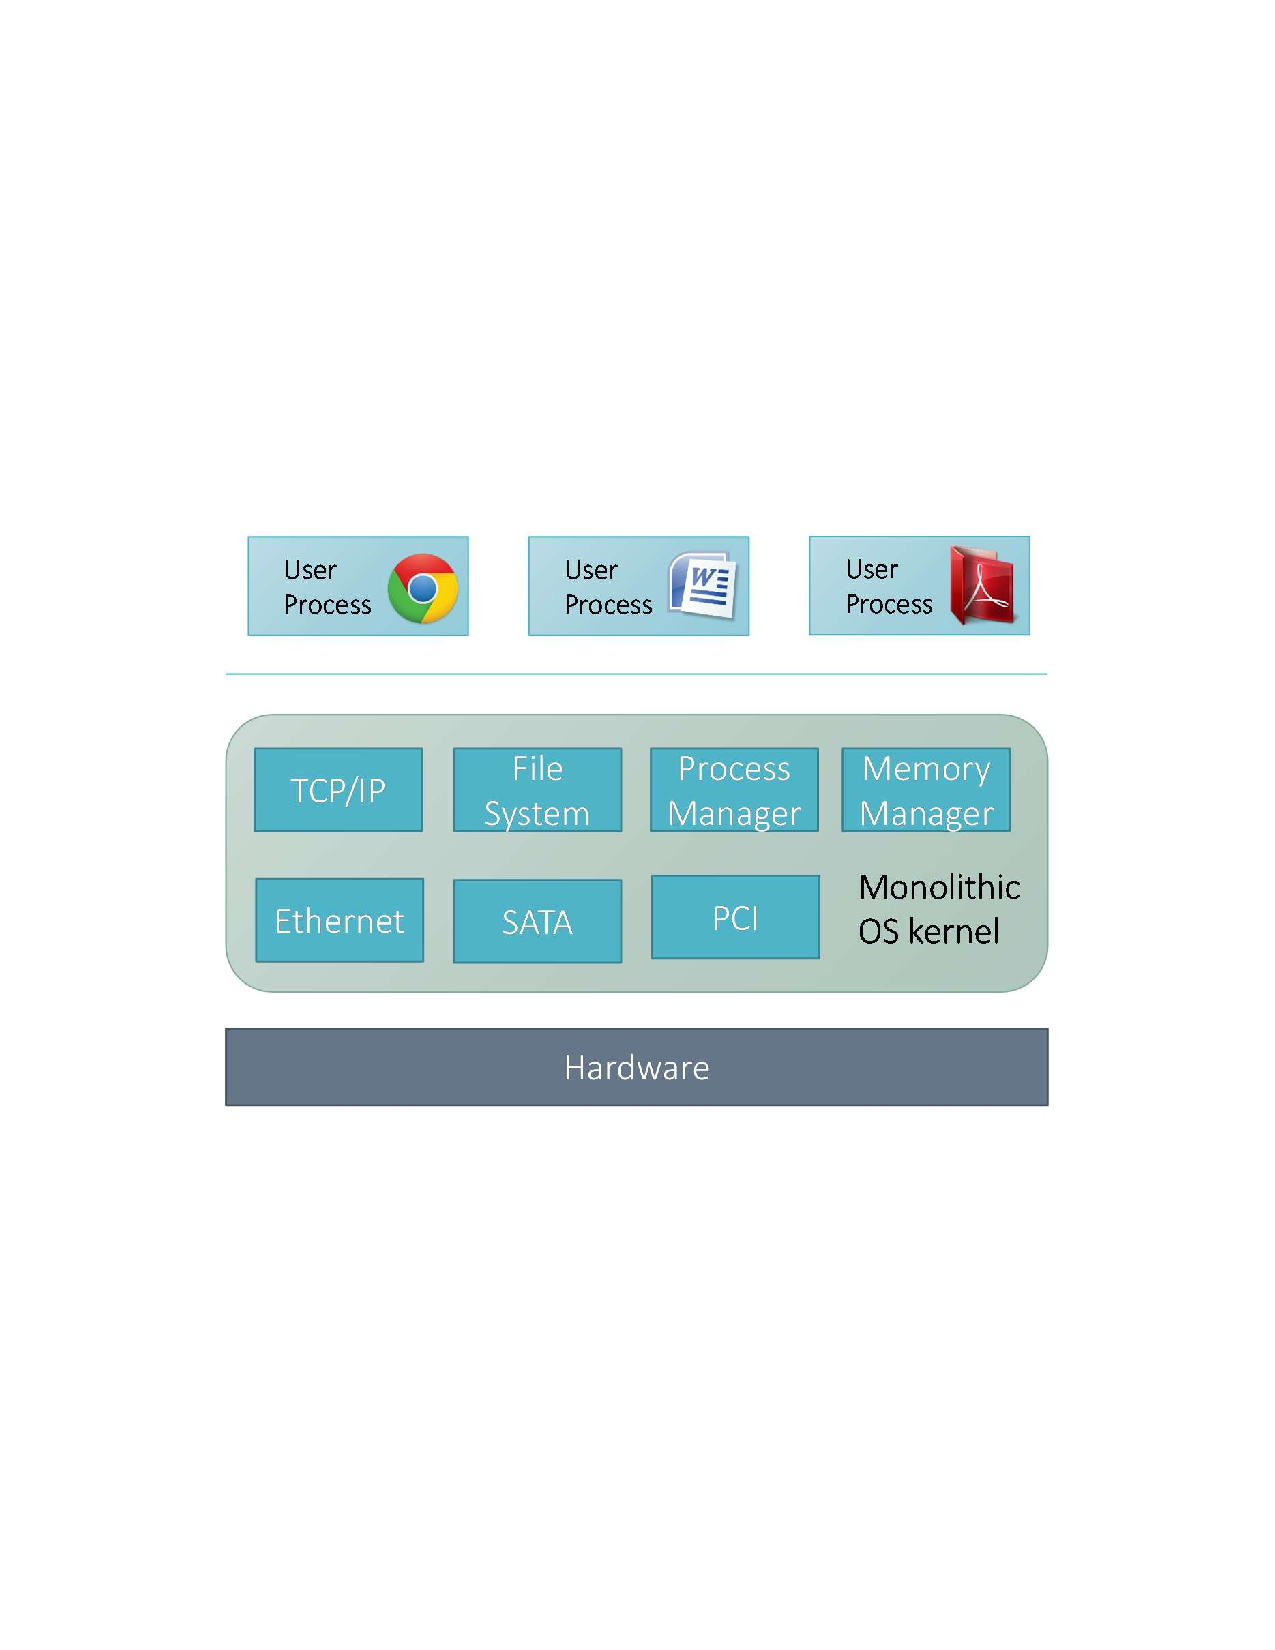
\includegraphics[scale=.5]{mem_ks1}
\caption{Kernel space}
\label{fig:Kernel space1}
\end{figure}

\begin{enumerate}
\item In the system shown in figure~\ref{fig:Kernel space1}, Chromium browser, word processor and pdf reader are running as 3 different processes in the user space and many different kernel components are running.
\item The network driver hits a bug, and corrupts a kernel data structure. This memory corruption might crash the other components, and might lead to a system crash.
\item Ideally with proper memory protection policy implementation and proper decoupling between network device driver and kernel, only network device driver and applications using network device driver (chromium in this case) should have been crashed. 
\item But because of tight coupling between device driver and kernel, complete system crashes.
\end{enumerate}

\begin{figure}[!ht]
\centering
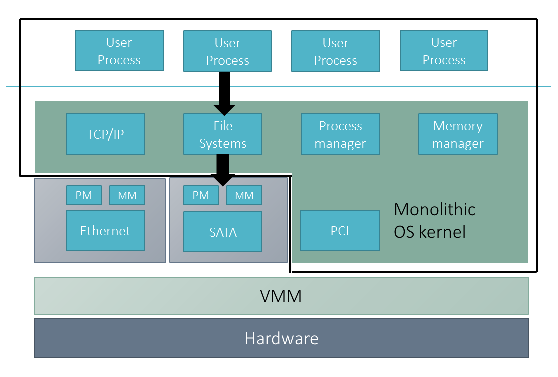
\includegraphics[scale=.5]{mem_ks2}
\caption{Kernel space}
\label{fig:Kernel space2}
\end{figure}

\begin{figure}[!ht]
\centering
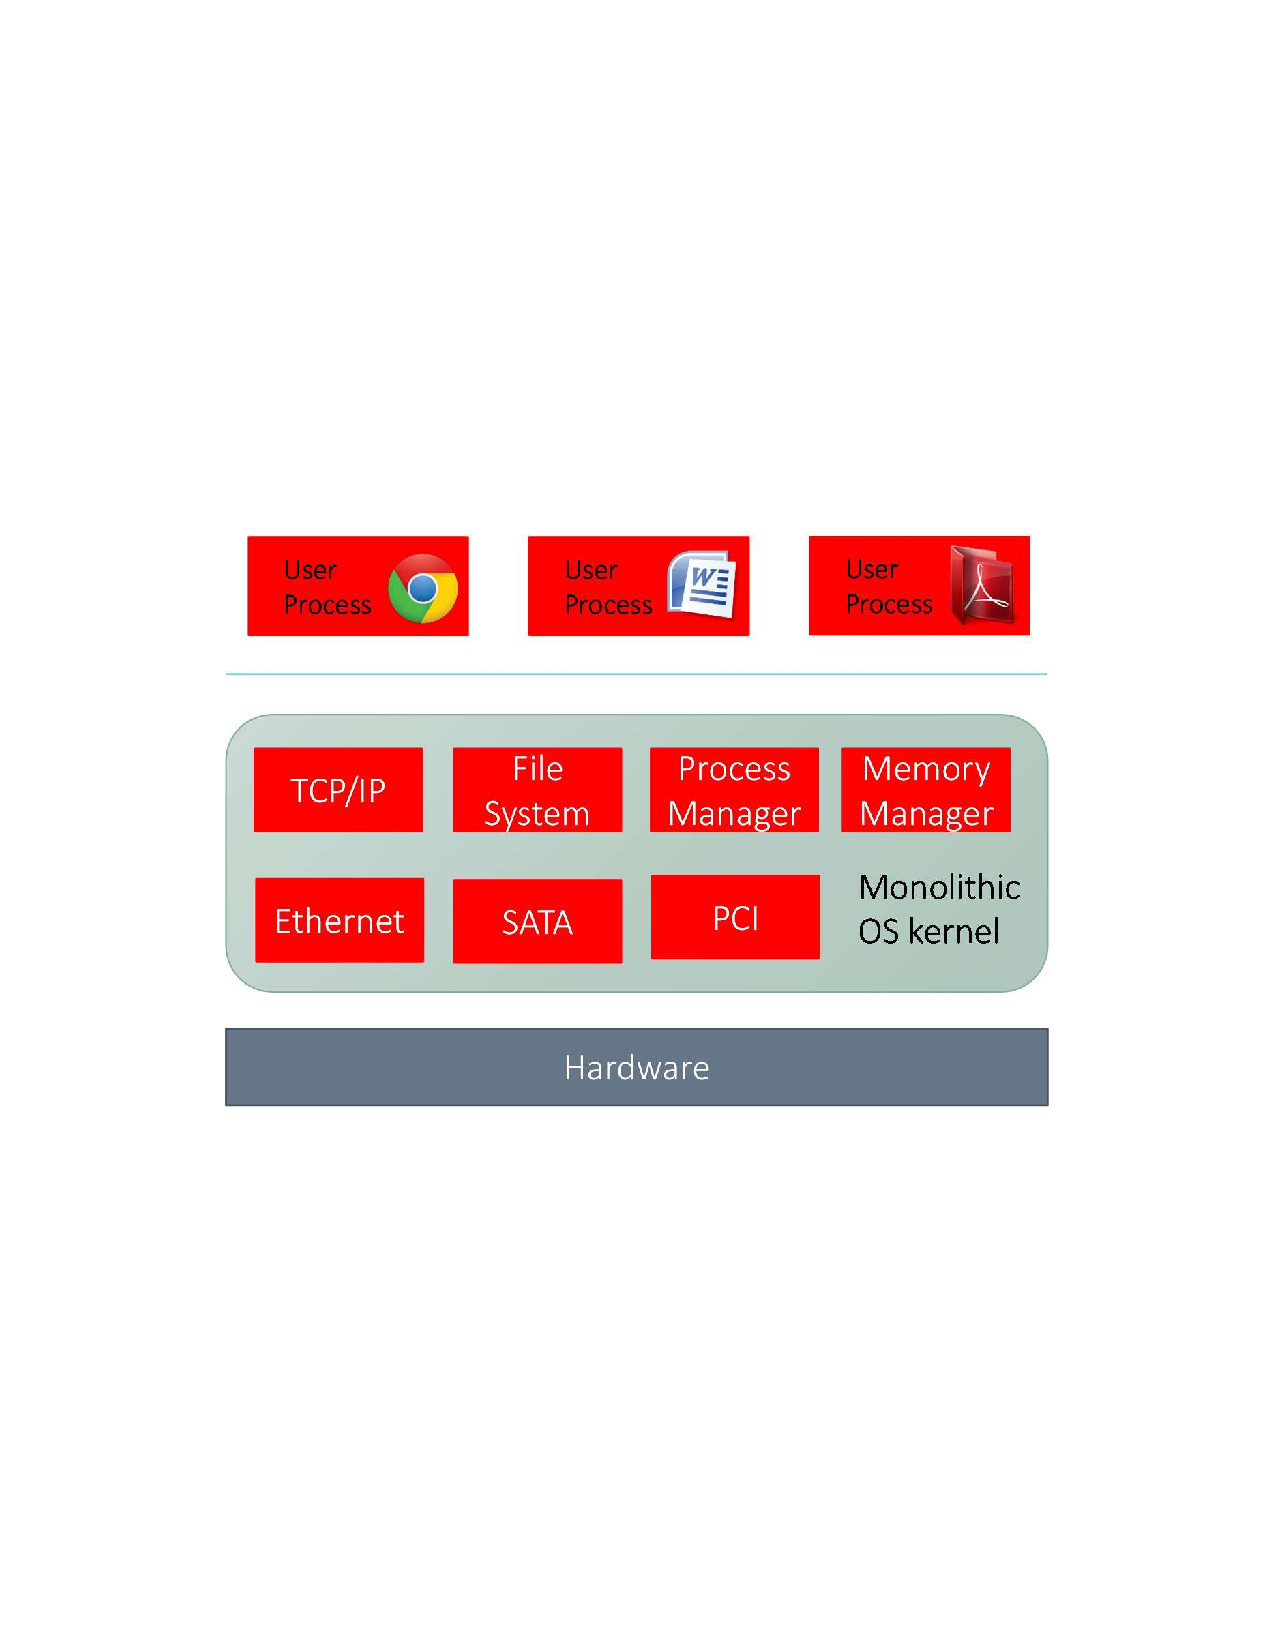
\includegraphics[scale=.5]{mem_ks3}
\caption{Kernel space}
\label{fig:Kernel space3}
\end{figure}


\clearpage
\section{Virtualization}

\begin{figure}[!ht]
\centering
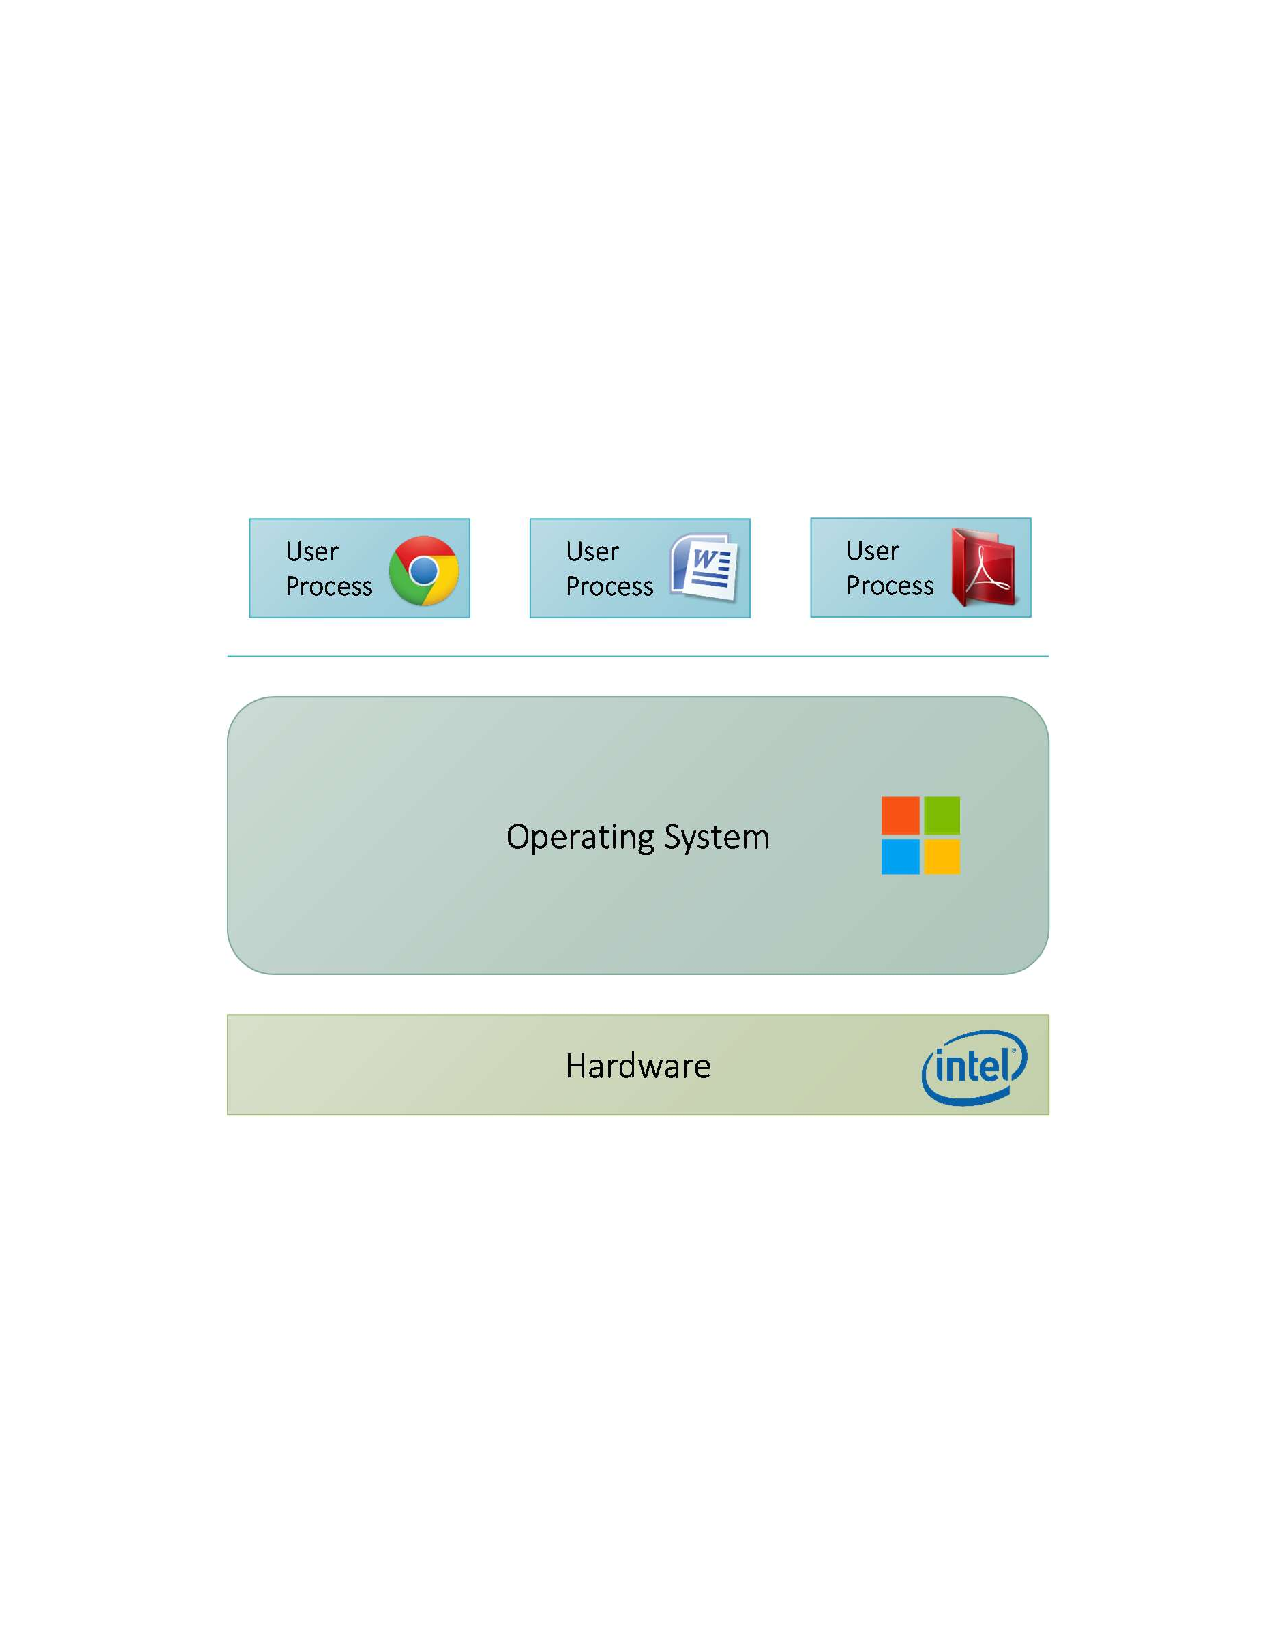
\includegraphics[scale=.5]{os1}
\caption{Operating System Architecture}
\label{fig:OS}
\end{figure}

Virtualization, is the act of creating a virtual version of hardware platform, operating system, storage device, or computer network resources etc. In operating system virtualization, the software allows a hardware to run multiple operating system images at the same time. Virtualization was invented to allow large expensive main frames to be easily shared among different application environments.\cite{Menascé05virtualization:concepts} Originally introduced for VM/370 \cite{Creasy:1981:OVT:1664853.1664863}, the idea later emerged for modern platforms \cite{Bugnion:1997:DRC:265924.265930, Rosenblum:2004:RVM:1016998.1017000}. 
\\
With the high hardware prices there was a need to share a single computer system between multiple users. This introduced the need to provide isolation between the users, which was achieved by providing the time-sharing systems. Virtualization concept started with the need to provide such isolation between users. 
\\
The addition of user and kernel modes on processors protected the operating system code from user programs. A set of privileged instructions reserved for the operating system software could run only in the kernel mode. The invention of Memory protection and later virtual memory made it possible to separate address spaces. The address space is assigned to different processes to share the system's physical memory and ensures that the use of memory is mutually exclusive by different applications. Before introduction of virtualization these enhancements were sufficient within an operating system. But the need to run different applications and users and different operating systems on a single physical machine could be satisfied only by virtualization.\cite{Crosby:2006:VR:1189276.1189289}
\\
Virtualization has the capability to share the underlying hardware resources and still provides isolated environment to each operating system. In virtualization each operating system runs independently from the other on its own virtual processors. Because of this isolation the failures in an operating system are contained. Virtualization is implemented in many different ways. It can be implemented either with or without hardware support. Also operating system might require some changes in order to run in a virtualized environment, or it can also function without making any changes.\cite{Drepper:2008:CV:1348583.1348591}. It has been shown that virtualization can be utilized to provide better security and robustness for operating systems\cite{Fraser04safehardware, LeVasseur04UnmodifiedDriverReuse, Riley:2008:GPK:1433006.1433008}.

\subsection{Hypervisor}

Hypervisor is a piece of computer software, firmware or hardware that creates and runs virtual machines. Operating system virtualization is achieved by inserting a hypervisor between the guest operating system and the underlying hardware. Most of the literature presents hypervisor synonymous to virtual machine monitor (VMM). While, VMM is a software layer specifically responsible for virtualizing a given architecture, a hypervisor is an operating system with a VMM. The operating system may be a general purpose one, such as Linux, or it may be developed specifically for the purpose of running virtual machines\cite{Agesen:2010:EXV:1899928.1899930}.
\\
A computer on which a hypervisor is running one or more virtual machines, is defined as a host machine. Each virtual machine is called a guest machine. The hypervisor presents the guest operating systems with a virtual operating platform and manages the execution of the guest operating systems. Multiple instances of a variety of operating systems may share the virtualized hardware resources. Among widely known hypervisors are Xen \cite{Barham:2003:XAV:1165389.945462, Chisnall:2007:DGX:1407351}, KVM\cite{Habib:2008:VK:1344209.1344217, kivity07kvm}, VMware ESX\cite{Agesen:2010:EXV:1899928.1899930},and VirtualBox\cite{citeulike:3149886}.
\\
\begin{figure}[!ht]
\centering
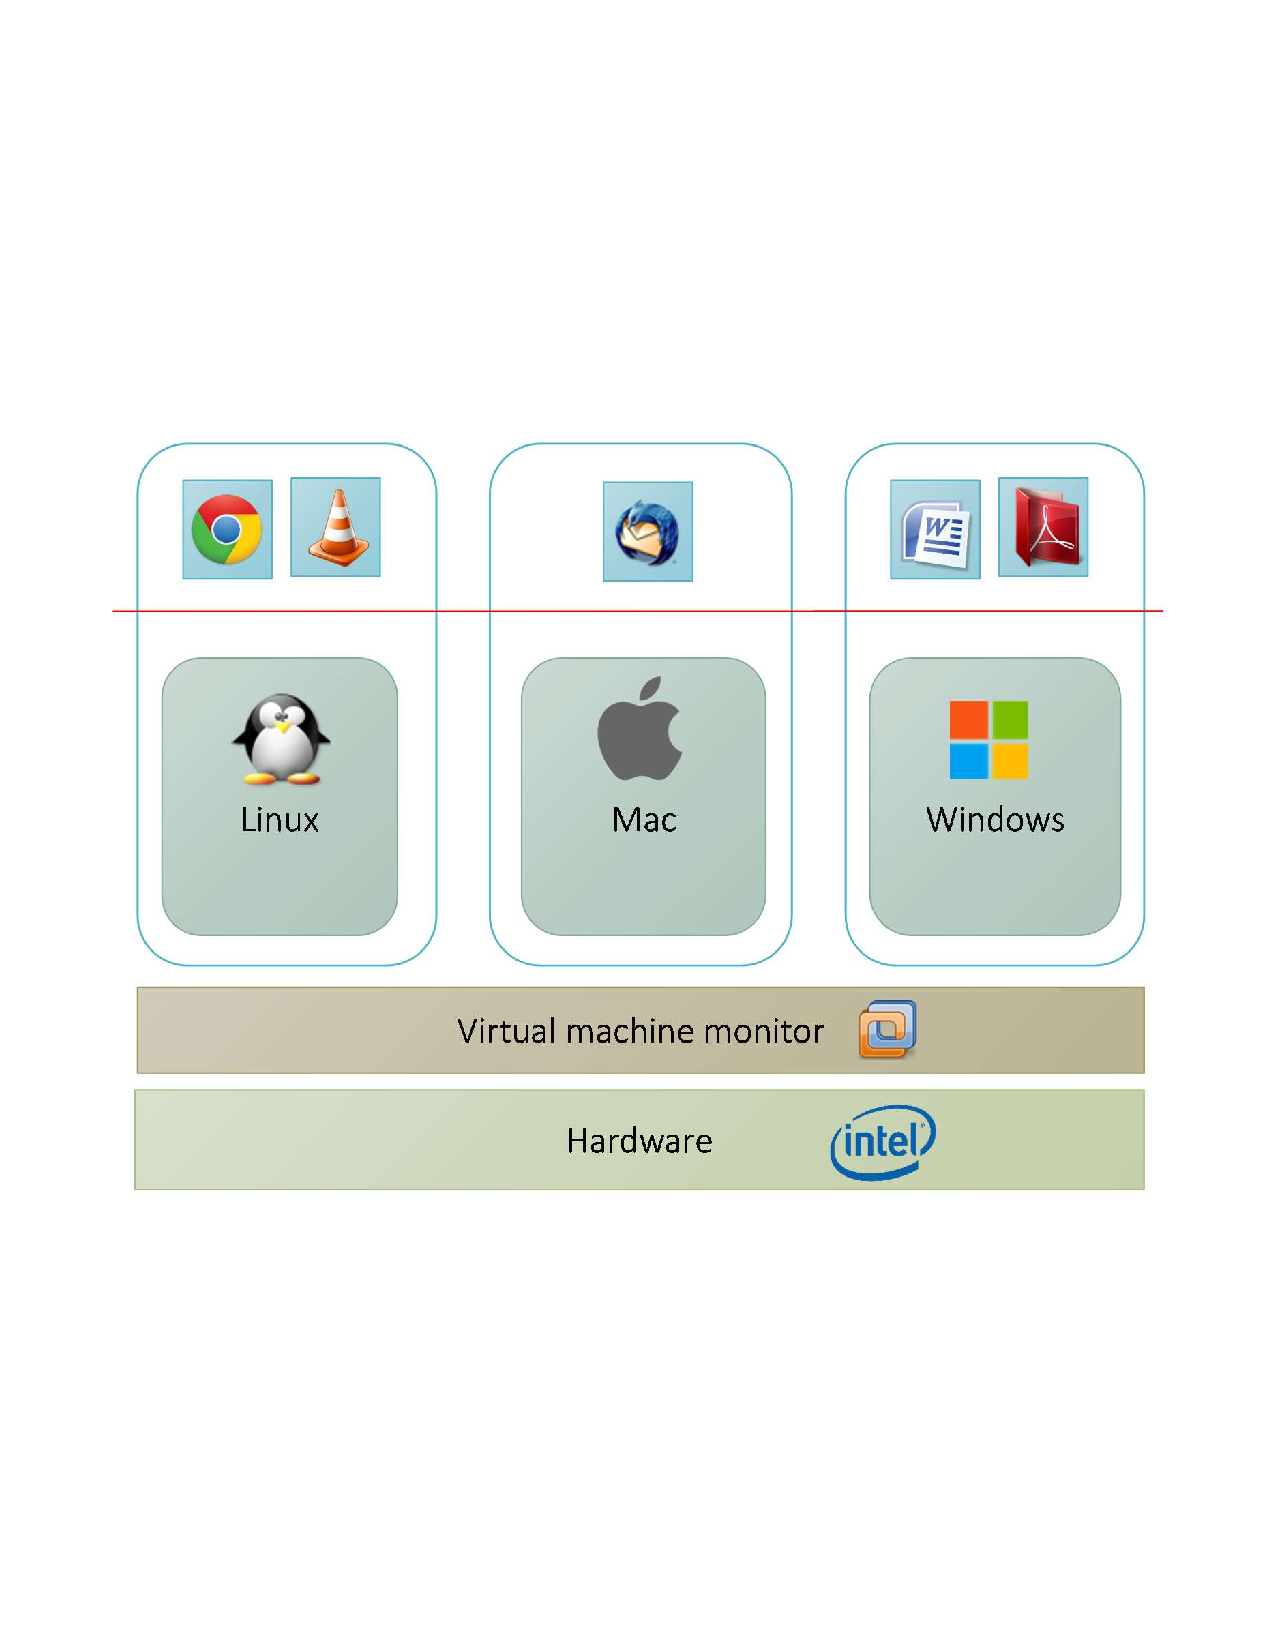
\includegraphics[scale=.5]{os2}
\caption{Virtualization}
\label{fig:Virtualization}
\end{figure}
There are two types of hypervisors \cite{Goldberg:1973:AVM:800122.803950}
\begin{description}
\item Type 1 hypervisors are also called as native hypervisors or bare metal hypervisors. Type 1 hypervisor runs directly on the host's hardware to control the hardware and to manage guest operating systems. A guest operating-system, thus, runs on another level above the hypervisor. Type 1 hypervisor represents the classic implementation of virtual-machine architectures such as SIMMON, and CP/CMS. Modern equivalents include Oracle VM Server for SPARC, Oracle VM Server, the Xen hypervisor\cite{Barham:2003:XAV:1165389.945462}, VMware ESX/ESXi\cite{Agesen:2010:EXV:1899928.1899930} and Microsoft Hyper-V.
\end{description}
\begin{figure}[!ht]
\centering
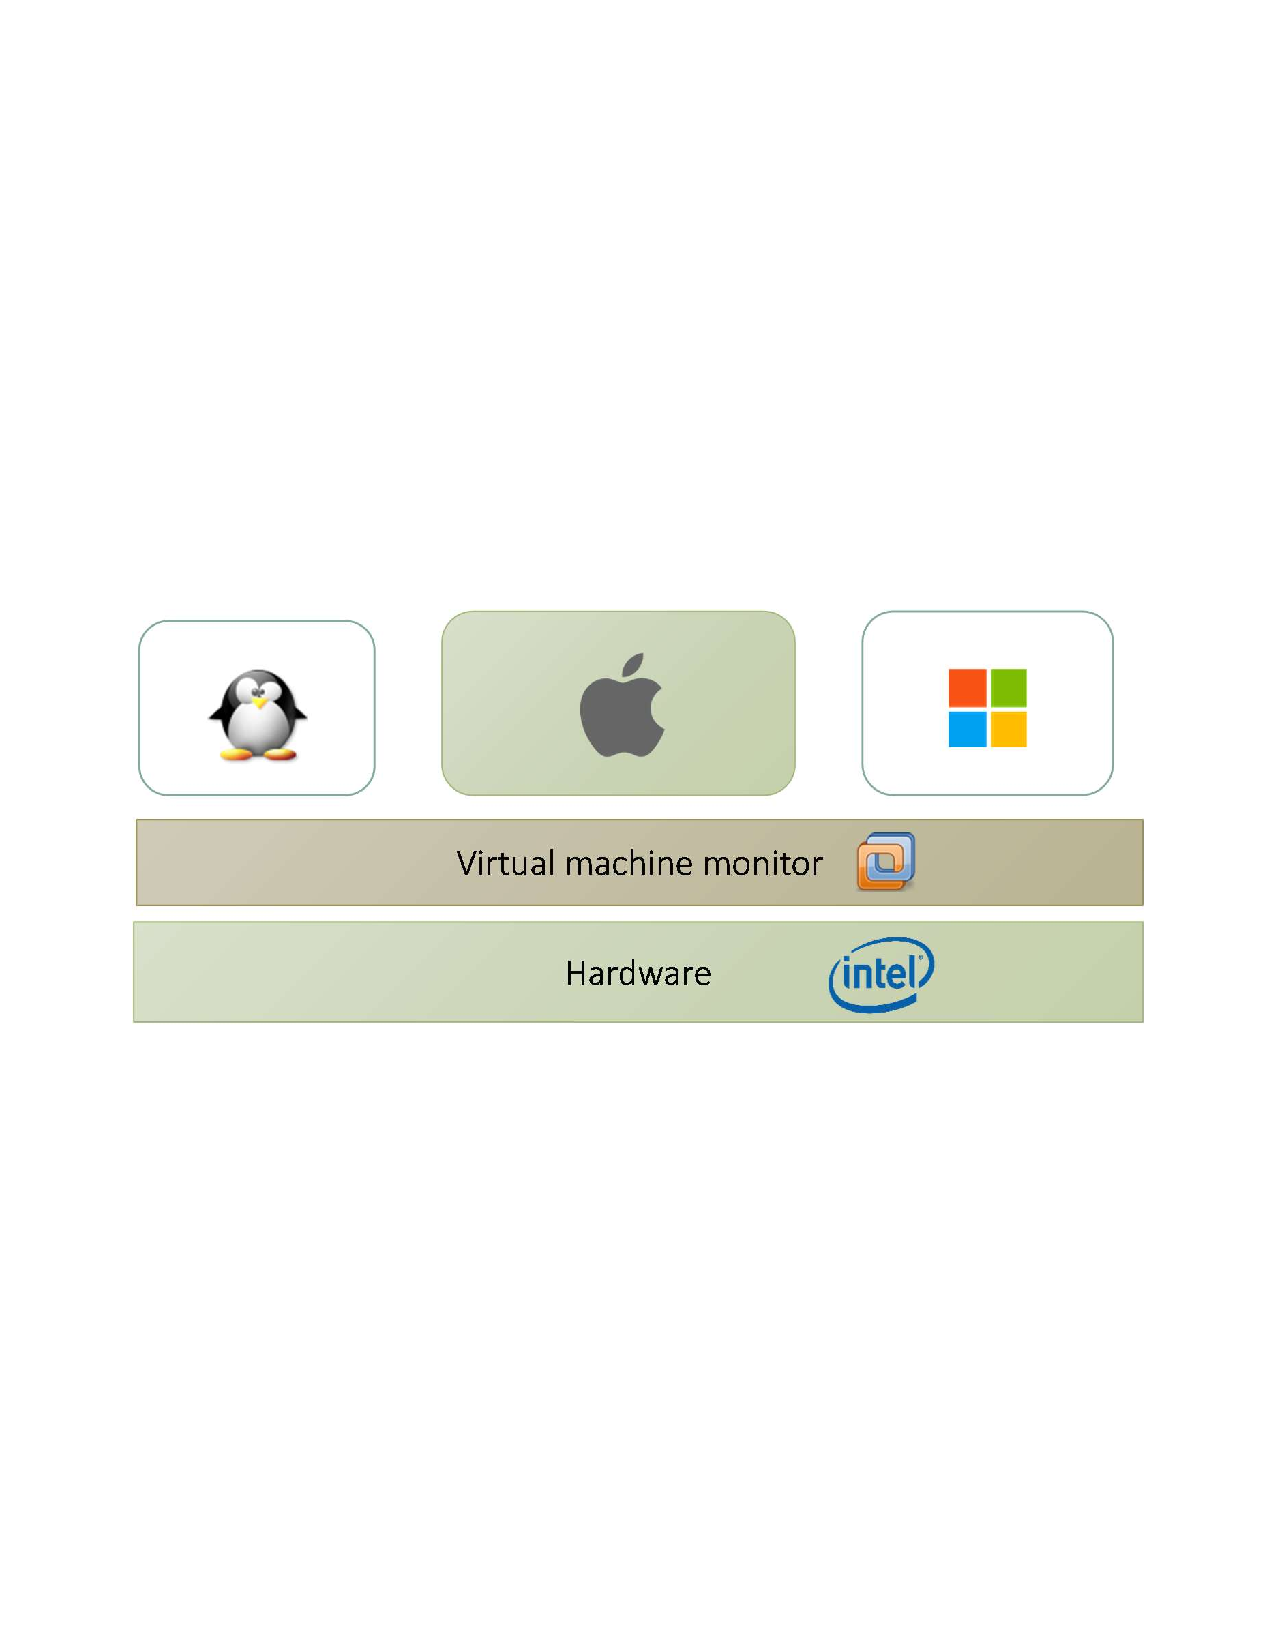
\includegraphics[scale=.5]{hypervisor_t2}
\caption{Type 1 hypervisor}
\label{Type 1 hypervisor}
\end{figure}
\begin{description}
\item Type 2 hypervisors are also called as hosted hypervisors. Type 2 hypervisor runs within a conventional operating-system environment. Type 2 hypervisor runs at a distinct second software level whereas, guest operating systems run at the third level above hardware. VMware Workstation and VirtualBox are some of the examples of Type 2 hypervisors\cite{Sugerman:2001:VID:647055.715774, citeulike:3149886}.
\end{description}
\begin{figure}[!ht]
\centering
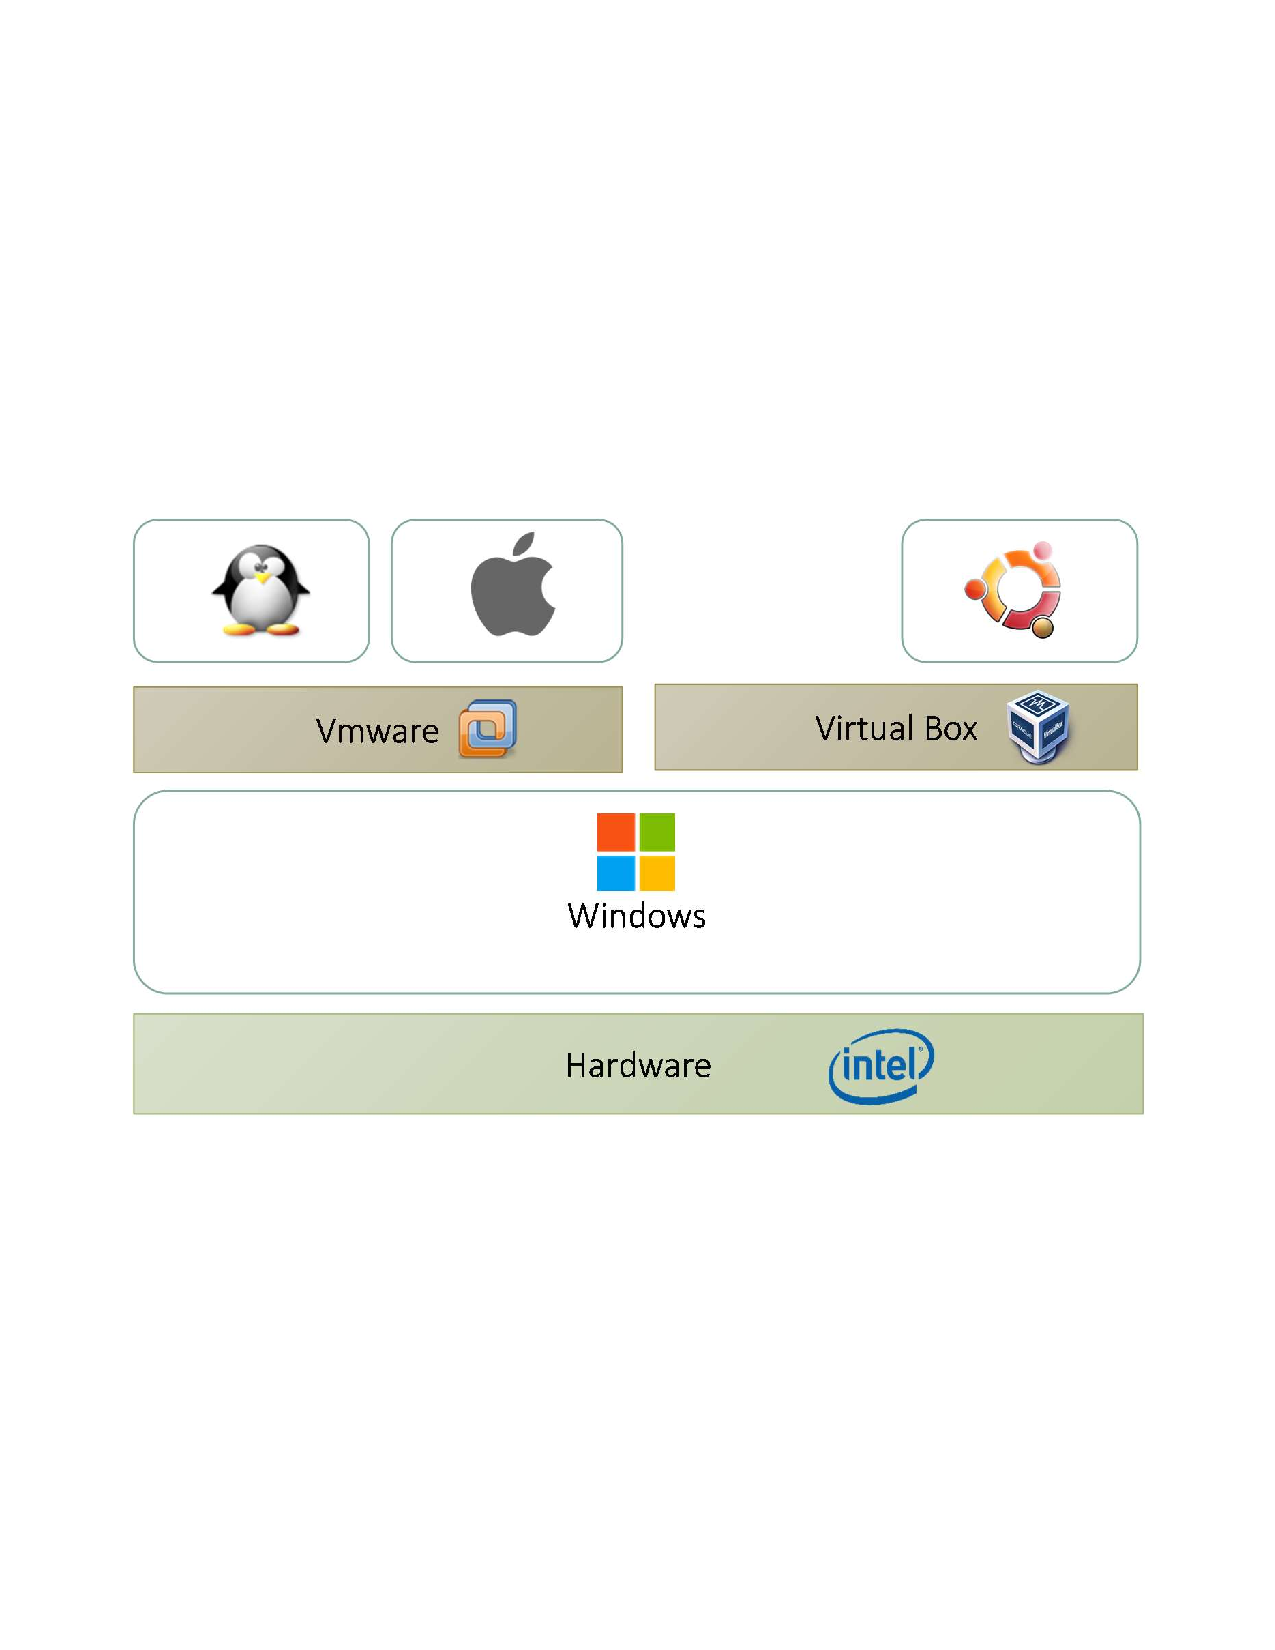
\includegraphics[scale=.5]{hypervisor_t1}
\caption{Type 2 hypervisor}
\label{Type 2 hypervisor}
\end{figure}

\subsection{Xen Hypervisor}

Xen\cite{Barham:2003:XAV:1165389.945462} is a widely known Type I hypervisor that allows execution of virtual machines in guest domains\cite{King_operatingsystem}. Figure~\ref{fig:Type 2 hypervisor} represents a diagram showing the different layers of a Type I hypervisor system. The hypervisor itself forms the lowest layer, which consists of the hypervisor kernel and Virtual Machine Monitors. The kernel has direct access to the hardware and is responsible for resource allocation, resource scheduling and resource sharing. A hypervisor is a layer responsible for virtualizing and providing resources to a given operating system.
\\
The purpose of a hypervisor is to allow guests to be run. Xen runs guests in environments known as domains. Domain 0 is the first guest to run, and has elevated privileges. Xen loads a Domain 0 guest kernel during boot. Other unpriviledged domains are called as domain U. Xen hypervisor does not include device drivers. Device management is included in privileged domain $Dom 0$. $Dom 0$ uses the device drivers which are present in its guest kernel implementation. However, $dom U$ accesses devices using a split device driver architecture. In the split device architecture a front end driver in a guest domain communicates with a back end driver in $Dom 0$.
\\
Figure~\ref{xen-split2} shows what happens to a data when it is sent by an application running in a domU guest. First, it travels through the file system as it would normally. However, at the end of the stack the normal block device driver does not exist. Instead, a simple piece of code called the front end puts the data into the shared memory. The other half of the split device driver called the back end, running on the dom0 guest, reads the data from the buffer, sends it way down to the real device driver. The data is written on actual physical device. In conclusion, split device driver can be explained as a way to move data from the domU guests to the dom0 guest, usually using ring buffers in shared memory\cite{Chisnall:2007:DGX:1407351}.
\begin{figure}[!h]
\centering
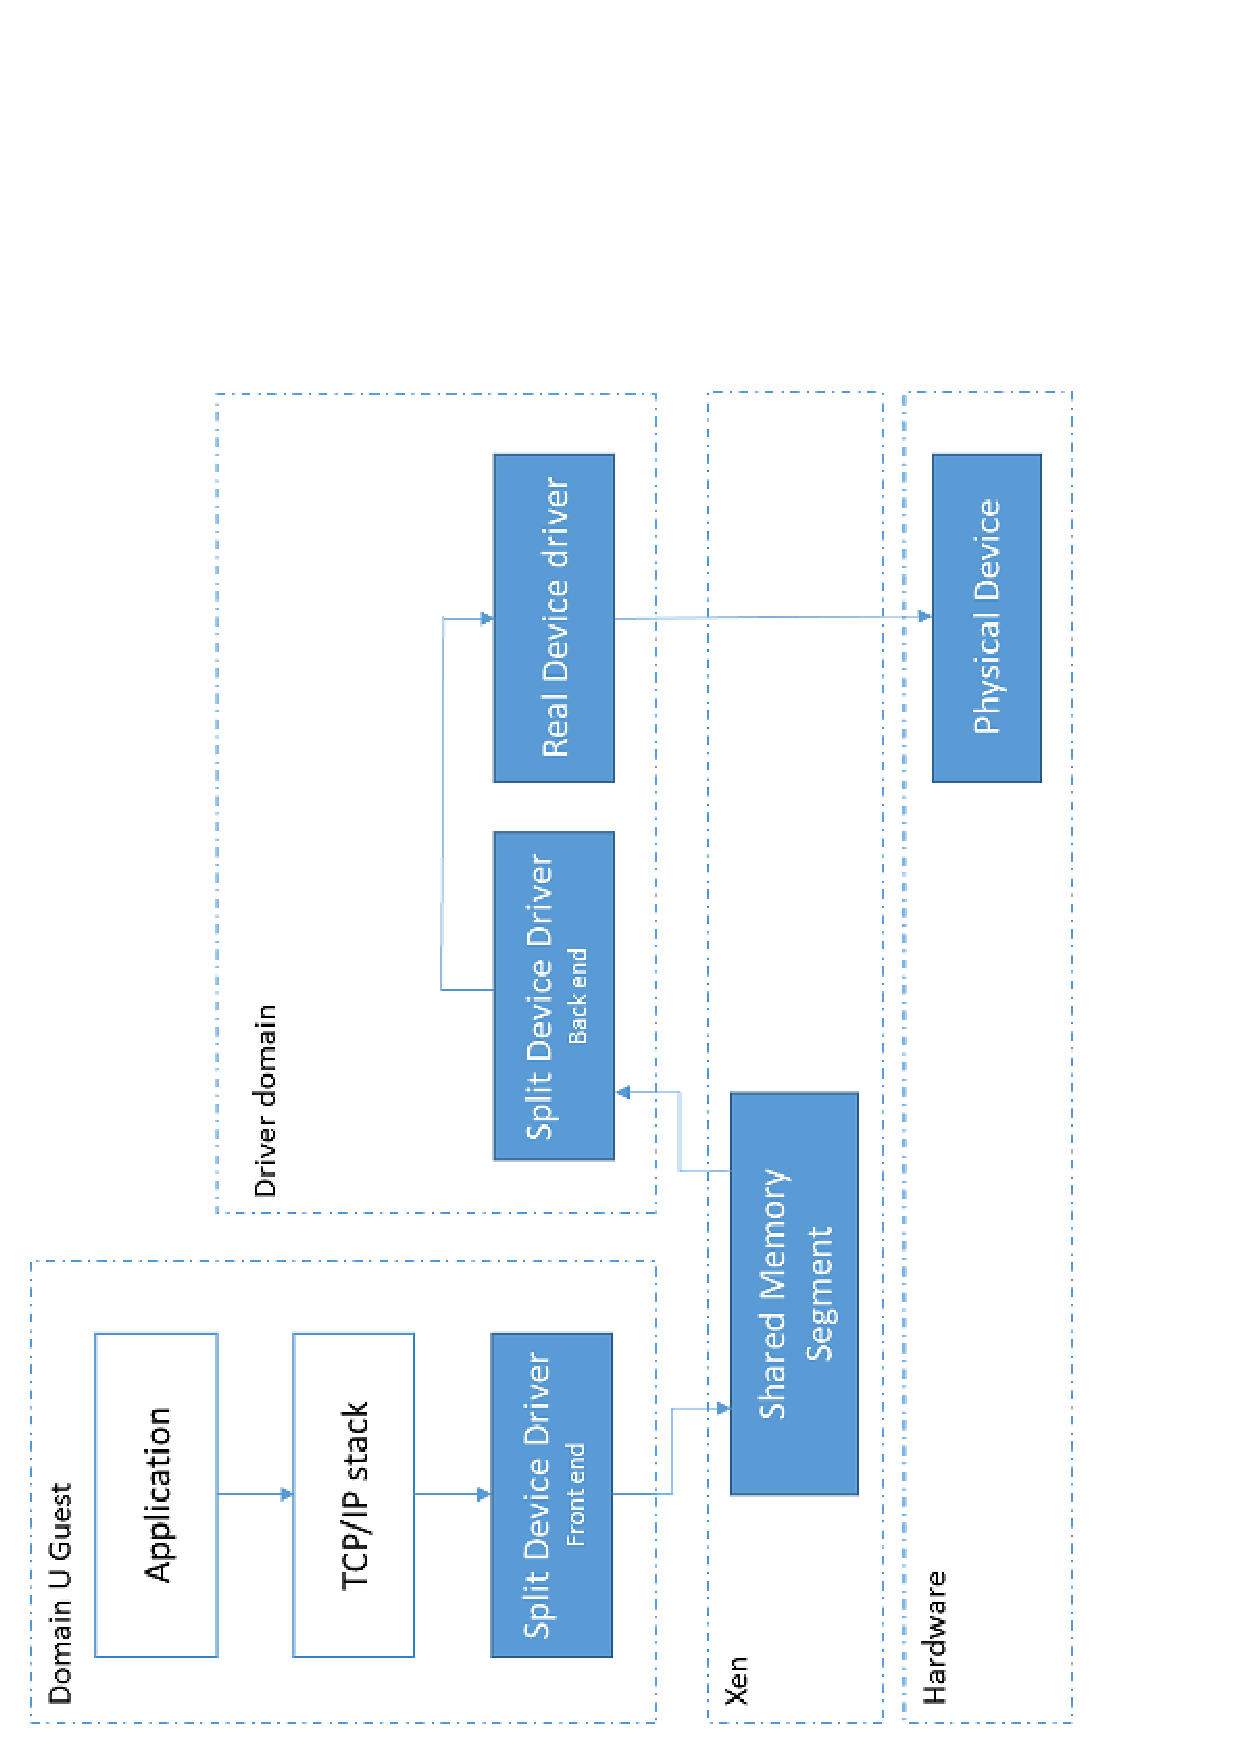
\includegraphics[scale=.40, angle=270]{xen-split}
\caption{Xen split device driver}
\label{xen-split2}
\end{figure}

Xen provides an inter-domain memory sharing API accessed through the guest kernel extensions, and an interrupt-based inter-domain signaling facility called event channels to implement the efficient inter-domain communication. Split drivers use memory sharing APIs to implement I/O device ring buffers to exchange data across domains.
\\
\begin{figure}[!h]
\centering
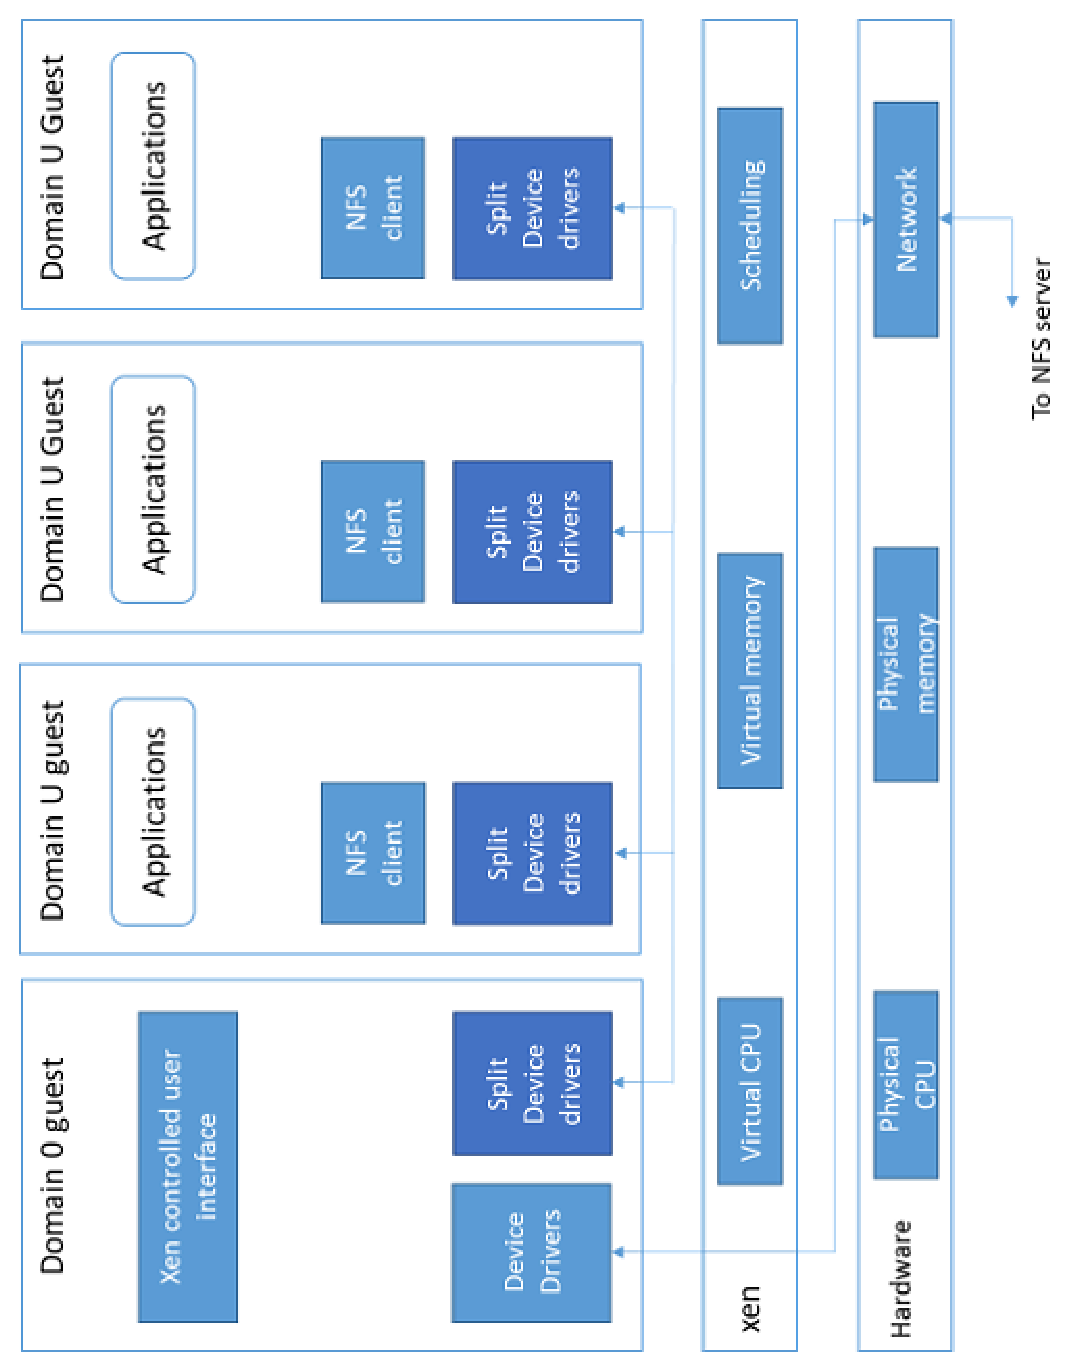
\includegraphics[scale=.40, angle=270]{xen}
\caption{Xen}
\label{xen}
\end{figure}

In driver domain implementation, xen uses shared I/O ring buffers and event channel\cite{Barham:2003:XAV:1165389.945462, Nikolaev:2013:VOS:2517349.2522719, Ruslan}.

\subsubsection{Hypercalls and events}

Hypercalls and event channels are two mechanisms that exist for interactions between Xen and domains. A hypercall is a software trap from a domain to the Xen, just as a syscall is a software trap from an application to the kernel\cite{hypercall}. Domains use the hypercalls to request privileged operations like updating pagetables. 
\\
Event channel is to Xen hypervisor as hardware interrupt is to operating system. Event channel is used for sending asynchronous notifications between domains. Event notifications are implemented by updating a bitmap. After scheduling pending events from an event queue, the event callback handler is called to take appropriate action. The callback handler is responsible for resetting the bitmap of pending events, and responding to the notifications in an appropriate manner. A domain may explicitly defer event handling by setting a Xen readable software flag: this is analogous to disabling interrupts on a real processor. Event notifications can be compared to traditional UNIX signals acting to flag a particular type of occurrence. For example, events are used to indicate that new data has been received over the network, or a virtual disk request has completed. 

\subsubsection{Data Transfer: I/O Rings}

Hypervisor introduces an additional layer between guest OS and I/O devices. Xen provides a data transfer mechanism that allows data to move vertically through the system with minimum overhead. Two main factors have shaped the design of I/O transfer mechanism which are resource management and event notification. 
\\*
\begin{figure}[!ht]
\centering
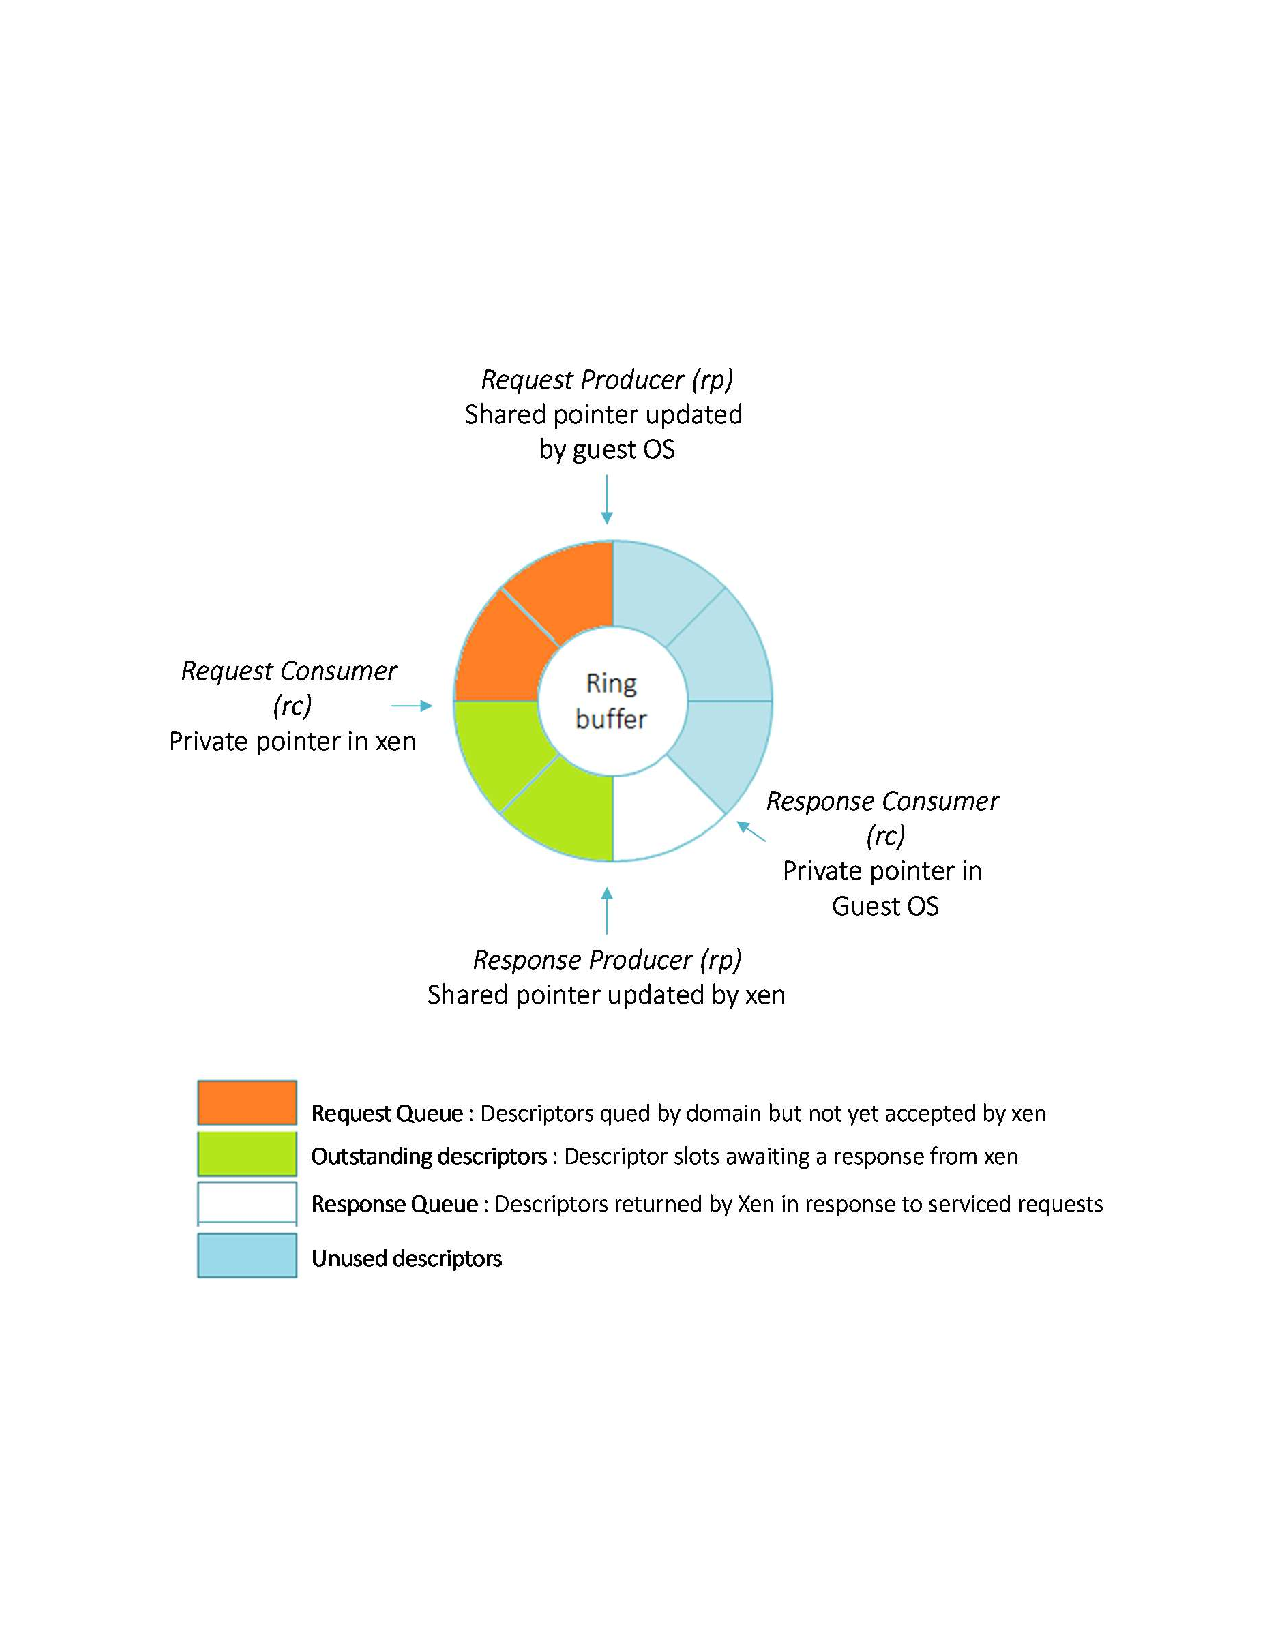
\includegraphics[scale=.5]{ring-buf}
\caption{Ring I/O buffer}
\label{fig:Ring buffer}
\end{figure}
Figure~\ref{fig:Ring buffer} shows the structure of I/O descriptor ring. I/O descriptor ring is a circular queue of descriptors allocated by a domain. These descriptors do not contain I/O data. However, I/O data buffers are allocated separately by the guest OS and is indirectly referenced by these I/O descriptors. Access to I/O ring is based around two pairs of producer-consumer pointers.

\begin{enumerate}
\item Request producer pointer: domains place requests on a ring by advancing request producer pointer. 
\item Request consumer pointer: Xen removes requests which are pointed by request producer pointer by advancing a request consumer pointer. 
\item Response producer pointer: Xen places responses on a ring by advancing response producer pointer. 
\item Response consumer pointer: Domains remove responses which are pointed by response producer pointer by advancing a response consumer pointer. 
\end{enumerate} 

The requests are not required to be processed in order. I/O rings are generic to support different device paradigms. For example, a set of $‘requests’$ can provide buffers for read data of virtual disks; subsequent $‘responses’$ then signal the arrival of data into these buffers. 
\\
The notification is not sent for production of each request and response. A domain can en-queue multiple requests and responses before notifying the other domain. This allows each domain to trade-off between latency and throughput.

\begin{figure}[!ht]
\centering
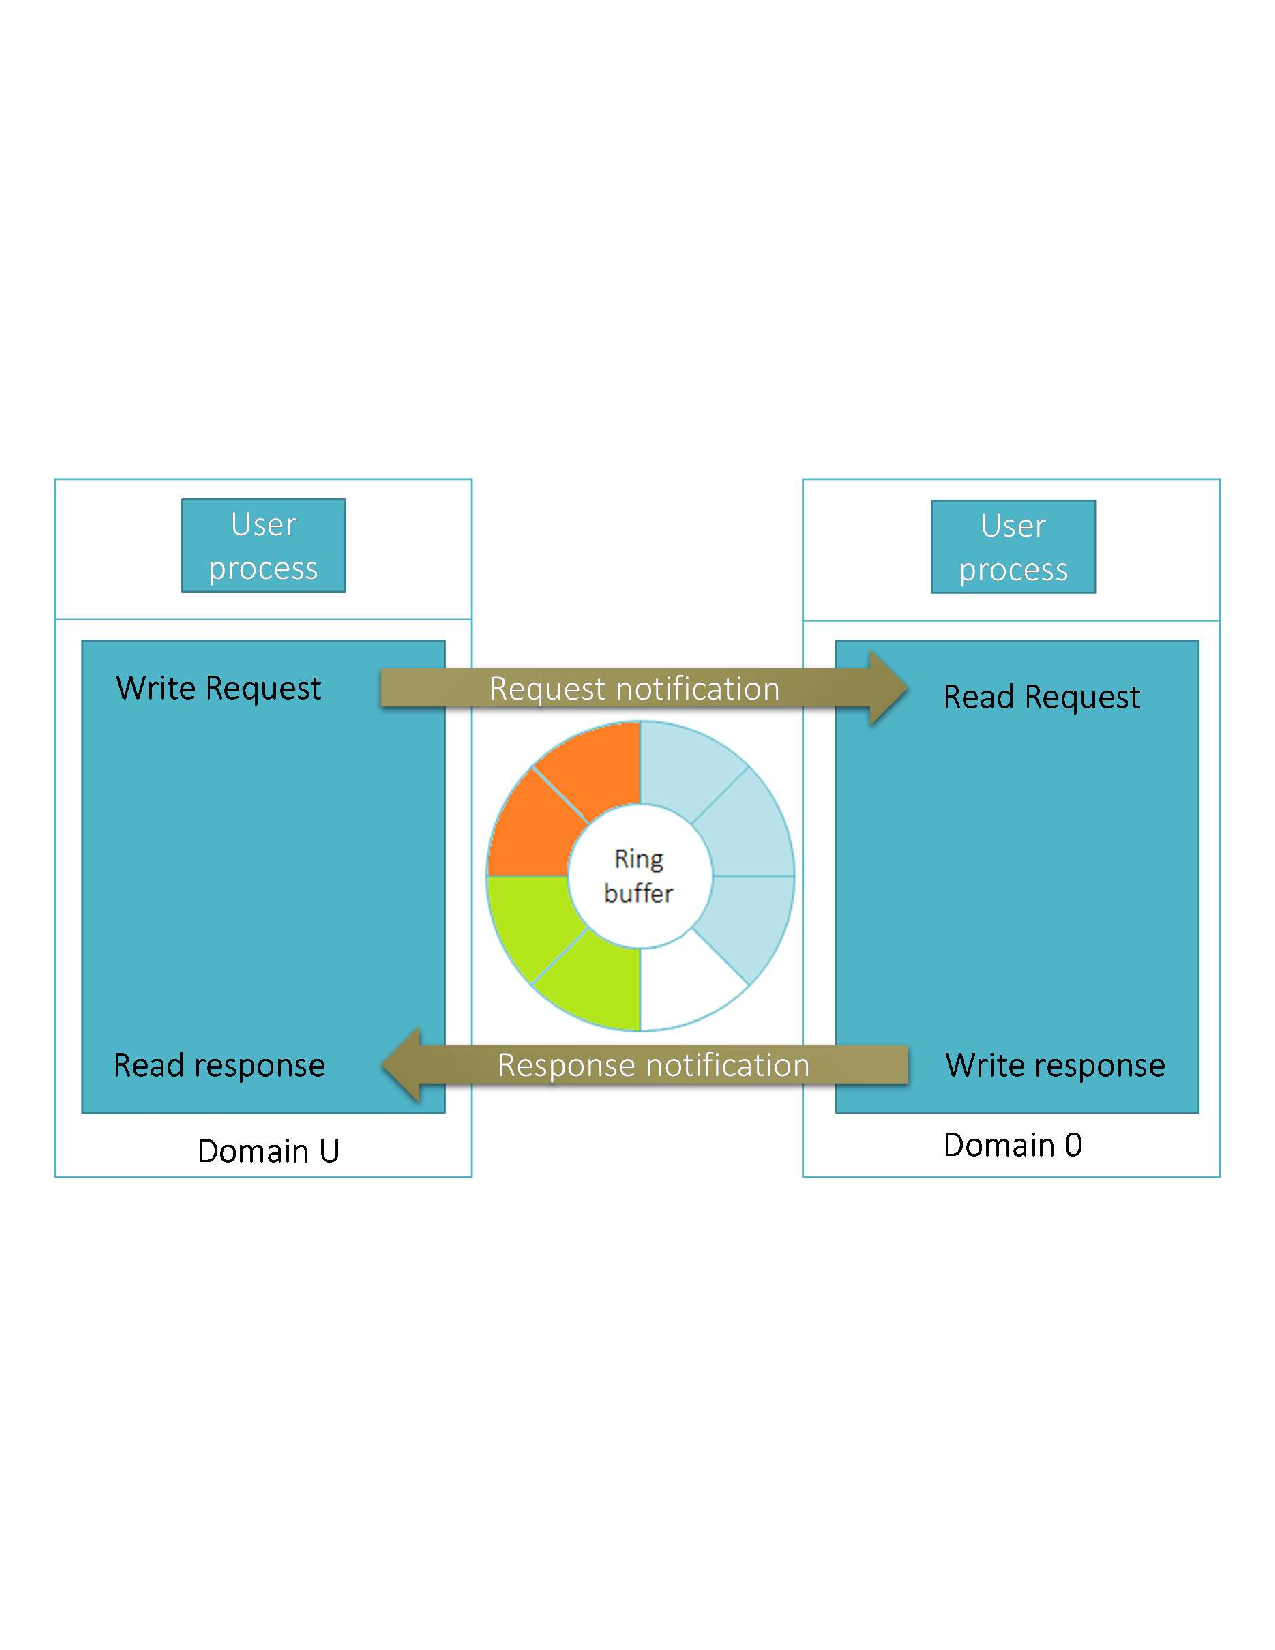
\includegraphics[scale=.5]{ring-buf2}
\caption{Ring I/O buffer}
\label{fig:Ring buffer}
\end{figure}
\pagebreak

\ifbool{toShowBibliography}{\bibliography{references}}{}
